\section{Conclusion}
This experiment was centered on building and testing the instrument known as the theremin. This involved designing and building several different sections from readily available materials and components such that they could be played as a traditional theremin, but also so that information and data could be collected regarding the performance, capabilities and characteristics of the final assembly.

This was completed up to and including the pitch control using two radio frequency voltage control oscillators, a mixer and a hand controlled parallel plate capacitor. The volume control would be implemented next using a very similar design as was used for the pitch control, but with a circuit to convert the change in frequency to a change in voltage which could be used to vary the amplitude, and so the volume, of the produced signal.

The final signal shape and quality of the VCO signals are shown in figure~\ref{fig:final}, and the final output is shown below in figure~\ref{fig:final out}

\begin{figure}[htb]
	\begin{center}
		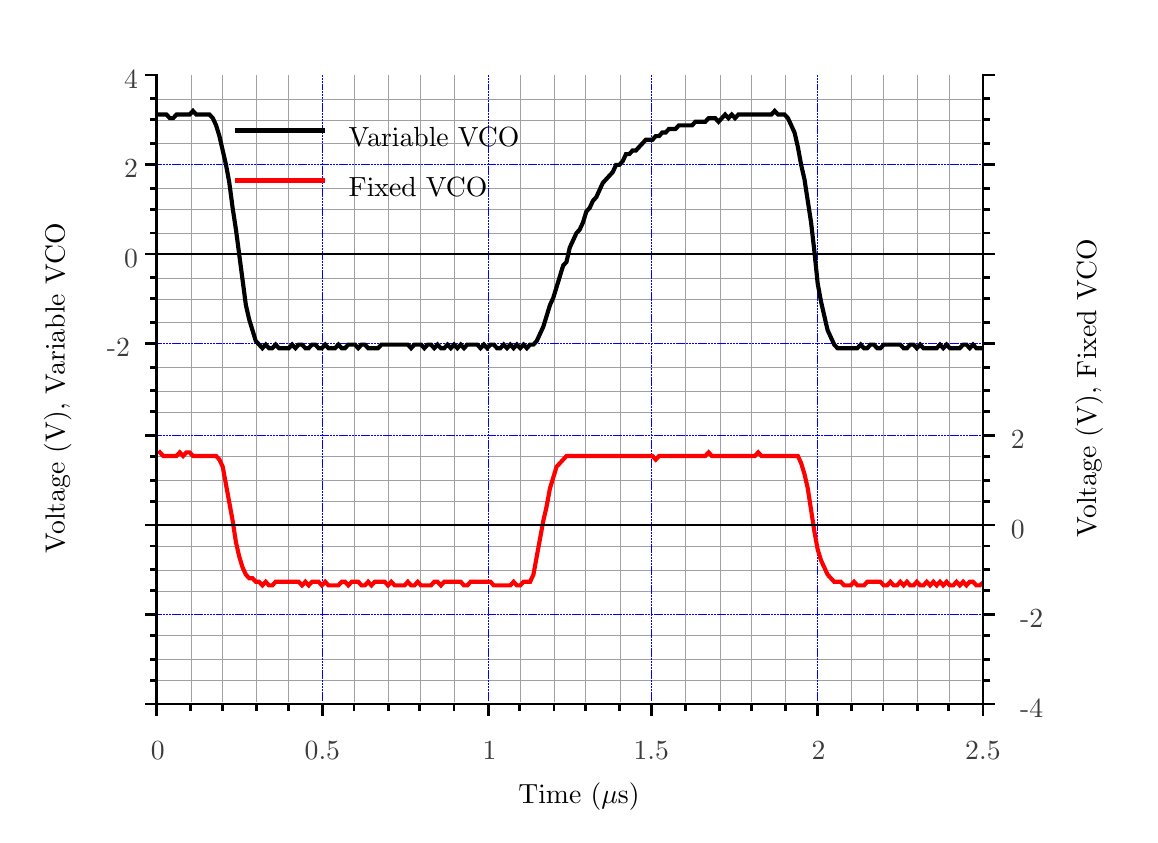
\begin{tikzpicture}{0pt}{0pt}{419pt}{299pt}
	\clip(0pt,299pt) -- (398.436pt,299pt) -- (398.436pt,14.6746pt) -- (0pt,14.6746pt) -- (0pt,299pt);
\begin{scope}
	\clip(46.5951pt,281.883pt) -- (345.184pt,281.883pt) -- (345.184pt,54.6133pt) -- (46.5951pt,54.6133pt) -- (46.5951pt,281.883pt);
	\color[rgb]{0.627451,0.627451,0.643137}
	\draw[line width=0.1pt, dash pattern=on 0.0024cm off 0.008cm, dash phase=0pt, line join=bevel, line cap=rect](58.9571pt,281.883pt) -- (58.9571pt,55.5642pt);
	\color[rgb]{0.627451,0.627451,0.643137}
	\draw[line width=0.1pt, dash pattern=on 0.0024cm off 0.008cm, dash phase=0pt, line join=bevel, line cap=rect](70.3682pt,281.883pt) -- (70.3682pt,55.5642pt);
	\draw[line width=0.1pt, dash pattern=on 0.0024cm off 0.008cm, dash phase=0pt, line join=bevel, line cap=rect](82.7301pt,281.883pt) -- (82.7301pt,55.5642pt);
	\draw[line width=0.1pt, dash pattern=on 0.0024cm off 0.008cm, dash phase=0pt, line join=bevel, line cap=rect](94.1412pt,281.883pt) -- (94.1412pt,55.5642pt);
	\draw[line width=0.1pt, dash pattern=on 0.0024cm off 0.008cm, dash phase=0pt, line join=bevel, line cap=rect](117.914pt,281.883pt) -- (117.914pt,55.5642pt);
	\draw[line width=0.1pt, dash pattern=on 0.0024cm off 0.008cm, dash phase=0pt, line join=bevel, line cap=rect](130.276pt,281.883pt) -- (130.276pt,55.5642pt);
	\draw[line width=0.1pt, dash pattern=on 0.0024cm off 0.008cm, dash phase=0pt, line join=bevel, line cap=rect](141.687pt,281.883pt) -- (141.687pt,55.5642pt);
	\draw[line width=0.1pt, dash pattern=on 0.0024cm off 0.008cm, dash phase=0pt, line join=bevel, line cap=rect](154.049pt,281.883pt) -- (154.049pt,55.5642pt);
	\draw[line width=0.1pt, dash pattern=on 0.0024cm off 0.008cm, dash phase=0pt, line join=bevel, line cap=rect](177.822pt,281.883pt) -- (177.822pt,55.5642pt);
	\draw[line width=0.1pt, dash pattern=on 0.0024cm off 0.008cm, dash phase=0pt, line join=bevel, line cap=rect](190.184pt,281.883pt) -- (190.184pt,55.5642pt);
	\draw[line width=0.1pt, dash pattern=on 0.0024cm off 0.008cm, dash phase=0pt, line join=bevel, line cap=rect](201.595pt,281.883pt) -- (201.595pt,55.5642pt);
	\draw[line width=0.1pt, dash pattern=on 0.0024cm off 0.008cm, dash phase=0pt, line join=bevel, line cap=rect](213.957pt,281.883pt) -- (213.957pt,55.5642pt);
	\draw[line width=0.1pt, dash pattern=on 0.0024cm off 0.008cm, dash phase=0pt, line join=bevel, line cap=rect](237.73pt,281.883pt) -- (237.73pt,55.5642pt);
	\draw[line width=0.1pt, dash pattern=on 0.0024cm off 0.008cm, dash phase=0pt, line join=bevel, line cap=rect](250.092pt,281.883pt) -- (250.092pt,55.5642pt);
	\draw[line width=0.1pt, dash pattern=on 0.0024cm off 0.008cm, dash phase=0pt, line join=bevel, line cap=rect](261.503pt,281.883pt) -- (261.503pt,55.5642pt);
	\draw[line width=0.1pt, dash pattern=on 0.0024cm off 0.008cm, dash phase=0pt, line join=bevel, line cap=rect](273.865pt,281.883pt) -- (273.865pt,55.5642pt);
	\draw[line width=0.1pt, dash pattern=on 0.0024cm off 0.008cm, dash phase=0pt, line join=bevel, line cap=rect](297.638pt,281.883pt) -- (297.638pt,55.5642pt);
	\draw[line width=0.1pt, dash pattern=on 0.0024cm off 0.008cm, dash phase=0pt, line join=bevel, line cap=rect](309.049pt,281.883pt) -- (309.049pt,55.5642pt);
	\draw[line width=0.1pt, dash pattern=on 0.0024cm off 0.008cm, dash phase=0pt, line join=bevel, line cap=rect](321.411pt,281.883pt) -- (321.411pt,55.5642pt);
	\draw[line width=0.1pt, dash pattern=on 0.0024cm off 0.008cm, dash phase=0pt, line join=bevel, line cap=rect](332.822pt,281.883pt) -- (332.822pt,55.5642pt);
	\draw[line width=0.1pt, dash pattern=on 0.0024cm off 0.008cm, dash phase=0pt, line join=bevel, line cap=rect](46.5951pt,63.1716pt) -- (344.233pt,63.1716pt);
	\draw[line width=0.1pt, dash pattern=on 0.0024cm off 0.008cm, dash phase=0pt, line join=bevel, line cap=rect](46.5951pt,79.3372pt) -- (344.233pt,79.3372pt);
	\draw[line width=0.1pt, dash pattern=on 0.0024cm off 0.008cm, dash phase=0pt, line join=bevel, line cap=rect](46.5951pt,95.5029pt) -- (344.233pt,95.5029pt);
	\draw[line width=0.1pt, dash pattern=on 0.0024cm off 0.008cm, dash phase=0pt, line join=bevel, line cap=rect](46.5951pt,111.669pt) -- (344.233pt,111.669pt);
	\draw[line width=0.1pt, dash pattern=on 0.0024cm off 0.008cm, dash phase=0pt, line join=bevel, line cap=rect](46.5951pt,127.834pt) -- (344.233pt,127.834pt);
	\draw[line width=0.1pt, dash pattern=on 0.0024cm off 0.008cm, dash phase=0pt, line join=bevel, line cap=rect](46.5951pt,144pt) -- (344.233pt,144pt);
	\draw[line width=0.1pt, dash pattern=on 0.0024cm off 0.008cm, dash phase=0pt, line join=bevel, line cap=rect](46.5951pt,160.166pt) -- (344.233pt,160.166pt);
	\draw[line width=0.1pt, dash pattern=on 0.0024cm off 0.008cm, dash phase=0pt, line join=bevel, line cap=rect](46.5951pt,176.331pt) -- (344.233pt,176.331pt);
	\draw[line width=0.1pt, dash pattern=on 0.0024cm off 0.008cm, dash phase=0pt, line join=bevel, line cap=rect](46.5951pt,192.497pt) -- (344.233pt,192.497pt);
	\draw[line width=0.1pt, dash pattern=on 0.0024cm off 0.008cm, dash phase=0pt, line join=bevel, line cap=rect](46.5951pt,208.662pt) -- (344.233pt,208.662pt);
	\draw[line width=0.1pt, dash pattern=on 0.0024cm off 0.008cm, dash phase=0pt, line join=bevel, line cap=rect](46.5951pt,224.828pt) -- (344.233pt,224.828pt);
	\draw[line width=0.1pt, dash pattern=on 0.0024cm off 0.008cm, dash phase=0pt, line join=bevel, line cap=rect](46.5951pt,240.994pt) -- (344.233pt,240.994pt);
	\draw[line width=0.1pt, dash pattern=on 0.0024cm off 0.008cm, dash phase=0pt, line join=bevel, line cap=rect](46.5951pt,257.159pt) -- (344.233pt,257.159pt);
	\draw[line width=0.1pt, dash pattern=on 0.0024cm off 0.008cm, dash phase=0pt, line join=bevel, line cap=rect](46.5951pt,273.325pt) -- (344.233pt,273.325pt);
	\draw[line width=0.1pt, dash pattern=on 0.0024cm off 0.008cm, dash phase=0pt, line join=bevel, line cap=rect](46.5951pt,70.7789pt) -- (344.233pt,70.7789pt);
	\draw[line width=0.1pt, dash pattern=on 0.0024cm off 0.008cm, dash phase=0pt, line join=bevel, line cap=rect](46.5951pt,103.11pt) -- (344.233pt,103.11pt);
	\draw[line width=0.1pt, dash pattern=on 0.0024cm off 0.008cm, dash phase=0pt, line join=bevel, line cap=rect](46.5951pt,135.442pt) -- (344.233pt,135.442pt);
	\draw[line width=0.1pt, dash pattern=on 0.0024cm off 0.008cm, dash phase=0pt, line join=bevel, line cap=rect](46.5951pt,167.773pt) -- (344.233pt,167.773pt);
	\draw[line width=0.1pt, dash pattern=on 0.0024cm off 0.008cm, dash phase=0pt, line join=bevel, line cap=rect](46.5951pt,201.055pt) -- (344.233pt,201.055pt);
	\draw[line width=0.1pt, dash pattern=on 0.0024cm off 0.008cm, dash phase=0pt, line join=bevel, line cap=rect](46.5951pt,233.386pt) -- (344.233pt,233.386pt);
	\draw[line width=0.1pt, dash pattern=on 0.0024cm off 0.008cm, dash phase=0pt, line join=bevel, line cap=rect](46.5951pt,265.718pt) -- (344.233pt,265.718pt);
	\color[rgb]{0,0,1}
	\draw[line width=0.2pt, dash pattern=on 0.024cm off 0.016cm, dash phase=0pt, line join=bevel, line cap=rect](106.503pt,281.883pt) -- (106.503pt,55.5642pt);
	\draw[line width=0.2pt, dash pattern=on 0.024cm off 0.016cm, dash phase=0pt, line join=bevel, line cap=rect](166.411pt,281.883pt) -- (166.411pt,55.5642pt);
	\draw[line width=0.2pt, dash pattern=on 0.024cm off 0.016cm, dash phase=0pt, line join=bevel, line cap=rect](225.368pt,281.883pt) -- (225.368pt,55.5642pt);
	\draw[line width=0.2pt, dash pattern=on 0.024cm off 0.016cm, dash phase=0pt, line join=bevel, line cap=rect](285.276pt,281.883pt) -- (285.276pt,55.5642pt);
	\draw[line width=0.2pt, dash pattern=on 0.024cm off 0.016cm, dash phase=0pt, line join=bevel, line cap=rect](46.5951pt,86.9446pt) -- (344.233pt,86.9446pt);
	\draw[line width=0.2pt, dash pattern=on 0.024cm off 0.016cm, dash phase=0pt, line join=bevel, line cap=rect](46.5951pt,119.276pt) -- (344.233pt,119.276pt);
	\draw[line width=0.2pt, dash pattern=on 0.024cm off 0.016cm, dash phase=0pt, line join=bevel, line cap=rect](46.5951pt,151.607pt) -- (344.233pt,151.607pt);
	\draw[line width=0.2pt, dash pattern=on 0.024cm off 0.016cm, dash phase=0pt, line join=bevel, line cap=rect](46.5951pt,184.889pt) -- (344.233pt,184.889pt);
	\draw[line width=0.2pt, dash pattern=on 0.024cm off 0.016cm, dash phase=0pt, line join=bevel, line cap=rect](46.5951pt,217.221pt) -- (344.233pt,217.221pt);
	\draw[line width=0.2pt, dash pattern=on 0.024cm off 0.016cm, dash phase=0pt, line join=bevel, line cap=rect](46.5951pt,249.552pt) -- (344.233pt,249.552pt);
	\color[rgb]{0,0,0}
	\draw[line width=1.5pt, line join=miter, line cap=rect](47.7895pt,267.598pt) -- (48.9838pt,267.598pt) -- (50.1782pt,267.598pt) -- (51.3726pt,266.299pt) -- (52.5669pt,266.299pt) -- (53.7613pt,267.598pt) -- (54.9556pt,267.598pt) -- (56.15pt,267.598pt) -- (57.3443pt,267.598pt) -- (58.5387pt,267.598pt) -- (59.7331pt,268.897pt) -- (60.9274pt,267.598pt) -- (62.1218pt,267.598pt) -- (63.3161pt,267.598pt) -- (64.5105pt,267.598pt) -- (65.7048pt,267.598pt) -- (66.8992pt,266.299pt) -- (68.0936pt,263.702pt) -- (69.2879pt,259.806pt) -- (70.4823pt,254.611pt) -- (71.6766pt,249.416pt) -- (72.871pt,242.923pt) -- (74.0653pt,233.832pt) -- (75.2597pt,226.04pt) -- (76.4541pt,216.949pt) -- (77.6484pt,207.858pt) -- (78.8428pt,198.767pt) -- (80.0371pt,193.573pt) -- (81.2315pt,189.677pt) -- (82.4258pt,185.781pt) -- (83.6202pt,184.482pt) -- (84.8146pt,183.183pt) -- (86.0089pt,184.482pt) -- (87.2033pt,183.183pt) -- (88.3976pt,183.183pt) -- (89.592pt,184.482pt) -- (90.7863pt,183.183pt) -- (91.9807pt,183.183pt) -- (93.175pt,183.183pt) -- (94.3694pt,183.183pt) -- (95.5638pt,184.482pt) -- (96.7581pt,183.183pt) -- (97.9525pt,184.482pt) -- (99.1468pt,184.482pt) -- (100.341pt,183.183pt) -- (101.536pt,183.183pt) -- (102.73pt,184.482pt) -- (103.924pt,184.482pt) -- (105.119pt,183.183pt) -- (106.313pt,183.183pt) -- (107.507pt,184.482pt) -- (108.702pt,183.183pt) -- (109.896pt,183.183pt) -- (111.09pt,183.183pt) -- (112.285pt,184.482pt) -- (113.479pt,183.183pt) -- (114.673pt,183.183pt) -- (115.868pt,184.482pt) -- (117.062pt,184.482pt) -- (118.257pt,184.482pt) -- (119.451pt,183.183pt) -- (120.645pt,184.482pt) -- (121.84pt,184.482pt) -- (123.034pt,183.183pt) -- (124.228pt,183.183pt) -- (125.423pt,183.183pt) -- (126.617pt,183.183pt) -- (127.811pt,184.482pt) -- (129.006pt,184.482pt) -- (130.2pt,184.482pt) -- (131.394pt,184.482pt) -- (132.589pt,184.482pt) -- (133.783pt,184.482pt) -- (134.978pt,184.482pt) -- (136.172pt,184.482pt) -- (137.366pt,184.482pt) -- (138.561pt,183.183pt) -- (139.755pt,184.482pt) -- (140.949pt,184.482pt) -- (142.144pt,184.482pt) -- (143.338pt,183.183pt) -- (144.532pt,184.482pt) -- (145.727pt,184.482pt) -- (146.921pt,183.183pt) -- (148.115pt,184.482pt) -- (149.31pt,183.183pt) -- (150.504pt,183.183pt) -- (151.699pt,184.482pt) -- (152.893pt,183.183pt) -- (154.087pt,184.482pt) -- (155.282pt,183.183pt) -- (156.476pt,184.482pt) -- (157.67pt,183.183pt) -- (158.865pt,184.482pt) -- (160.059pt,184.482pt) -- (161.253pt,184.482pt) -- (162.448pt,184.482pt) -- (163.642pt,183.183pt) -- (164.836pt,184.482pt) -- (166.031pt,183.183pt) -- (167.225pt,184.482pt) -- (168.42pt,184.482pt) -- (169.614pt,183.183pt) -- (170.808pt,183.183pt) -- (172.003pt,184.482pt) -- (173.197pt,183.183pt) -- (174.391pt,184.482pt) -- (175.586pt,183.183pt) -- (176.78pt,184.482pt) -- (177.974pt,183.183pt) -- (179.169pt,184.482pt) -- (180.363pt,183.183pt) -- (181.557pt,184.482pt) -- (182.752pt,184.482pt) -- (183.946pt,185.781pt) -- (185.141pt,188.378pt) -- (186.335pt,190.975pt) -- (187.529pt,194.871pt) -- (188.724pt,198.767pt) -- (189.918pt,201.365pt) -- (191.112pt,205.261pt) -- (192.307pt,209.157pt) -- (193.501pt,213.053pt) -- (194.695pt,214.352pt) -- (195.89pt,219.546pt) -- (197.084pt,222.144pt) -- (198.278pt,224.741pt) -- (199.473pt,226.04pt) -- (200.667pt,228.637pt) -- (201.862pt,232.533pt) -- (203.056pt,233.832pt) -- (204.25pt,236.429pt) -- (205.445pt,237.728pt) -- (206.639pt,240.325pt) -- (207.833pt,242.923pt) -- (209.028pt,244.222pt) -- (210.222pt,245.52pt) -- (211.416pt,246.819pt) -- (212.611pt,249.416pt) -- (213.805pt,249.416pt) -- (214.999pt,250.715pt) -- (216.194pt,253.312pt) -- (217.388pt,253.312pt) -- (218.583pt,254.611pt) -- (219.777pt,254.611pt) -- (220.971pt,255.91pt) -- (222.166pt,257.208pt) -- (223.36pt,258.507pt) -- (224.554pt,258.507pt) -- (225.749pt,258.507pt) -- (226.943pt,259.806pt) -- (228.137pt,259.806pt) -- (229.332pt,261.104pt) -- (230.526pt,261.104pt) -- (231.72pt,262.403pt) -- (232.915pt,262.403pt) -- (234.109pt,262.403pt) -- (235.304pt,263.702pt) -- (236.498pt,263.702pt) -- (237.692pt,263.702pt) -- (238.887pt,263.702pt) -- (240.081pt,263.702pt) -- (241.275pt,265pt) -- (242.47pt,265pt) -- (243.664pt,265pt) -- (244.858pt,265pt) -- (246.053pt,266.299pt) -- (247.247pt,266.299pt) -- (248.441pt,266.299pt) -- (249.636pt,265pt) -- (250.83pt,266.299pt) -- (252.025pt,267.598pt) -- (253.219pt,266.299pt) -- (254.413pt,267.598pt) -- (255.608pt,266.299pt) -- (256.802pt,267.598pt) -- (257.996pt,267.598pt) -- (259.191pt,267.598pt) -- (260.385pt,267.598pt) -- (261.579pt,267.598pt) -- (262.774pt,267.598pt) -- (263.968pt,267.598pt) -- (265.162pt,267.598pt) -- (266.357pt,267.598pt) -- (267.551pt,267.598pt) -- (268.746pt,267.598pt) -- (269.94pt,268.897pt) -- (271.134pt,267.598pt) -- (272.329pt,267.598pt) -- (273.523pt,267.598pt) -- (274.717pt,266.299pt) -- (275.912pt,263.702pt) -- (277.106pt,261.104pt) -- (278.3pt,255.91pt) -- (279.495pt,249.416pt) -- (280.689pt,244.222pt) -- (281.883pt,236.429pt) -- (283.078pt,228.637pt) -- (284.272pt,218.248pt) -- (285.466pt,206.56pt) -- (286.661pt,200.066pt) -- (287.855pt,194.871pt) -- (289.05pt,189.677pt) -- (290.244pt,187.079pt) -- (291.438pt,184.482pt) -- (292.633pt,183.183pt) -- (293.827pt,183.183pt) -- (295.021pt,183.183pt) -- (296.216pt,183.183pt) -- (297.41pt,183.183pt) -- (298.604pt,183.183pt) -- (299.799pt,183.183pt) -- (300.993pt,184.482pt) -- (302.187pt,183.183pt) -- (303.382pt,183.183pt) -- (304.576pt,184.482pt) -- (305.771pt,184.482pt) -- (306.965pt,183.183pt) -- (308.159pt,183.183pt) -- (309.354pt,184.482pt) -- (310.548pt,184.482pt) -- (311.742pt,184.482pt) -- (312.937pt,184.482pt) -- (314.131pt,184.482pt) -- (315.325pt,184.482pt) -- (316.52pt,183.183pt) -- (317.714pt,183.183pt) -- (318.908pt,184.482pt) -- (320.103pt,184.482pt) -- (321.297pt,183.183pt) -- (322.492pt,184.482pt) -- (323.686pt,183.183pt) -- (324.88pt,183.183pt) -- (326.075pt,183.183pt) -- (327.269pt,183.183pt) -- (328.463pt,183.183pt) -- (329.658pt,184.482pt) -- (330.852pt,183.183pt) -- (332.046pt,184.482pt) -- (333.241pt,183.183pt) -- (334.435pt,183.183pt) -- (335.629pt,183.183pt) -- (336.824pt,183.183pt) -- (338.018pt,184.482pt) -- (339.213pt,184.482pt) -- (340.407pt,183.183pt) -- (341.601pt,184.482pt) -- (342.796pt,183.183pt) -- (343.99pt,183.183pt) -- (345.184pt,183.183pt);
	\color[rgb]{1,0,0}
	\draw[line width=1.5pt, line join=miter, line cap=rect](47.7895pt,145.521pt) -- (48.9838pt,144.223pt) -- (50.1782pt,144.223pt) -- (51.3726pt,144.223pt) -- (52.5669pt,144.223pt) -- (53.7613pt,144.223pt) -- (54.9556pt,145.521pt) -- (56.15pt,144.223pt) -- (57.3443pt,145.521pt) -- (58.5387pt,145.521pt) -- (59.7331pt,144.223pt) -- (60.9274pt,144.223pt) -- (62.1218pt,144.223pt) -- (63.3161pt,144.223pt) -- (64.5105pt,144.223pt) -- (65.7048pt,144.223pt) -- (66.8992pt,144.223pt) -- (68.0936pt,144.223pt) -- (69.2879pt,142.924pt) -- (70.4823pt,140.327pt) -- (71.6766pt,133.833pt) -- (72.871pt,127.34pt) -- (74.0653pt,120.846pt) -- (75.2597pt,113.054pt) -- (76.4541pt,107.859pt) -- (77.6484pt,103.963pt) -- (78.8428pt,101.366pt) -- (80.0371pt,100.067pt) -- (81.2315pt,100.067pt) -- (82.4258pt,98.7686pt) -- (83.6202pt,98.7686pt) -- (84.8146pt,97.4699pt) -- (86.0089pt,98.7686pt) -- (87.2033pt,97.4699pt) -- (88.3976pt,97.4699pt) -- (89.592pt,98.7686pt) -- (90.7863pt,98.7686pt) -- (91.9807pt,98.7686pt) -- (93.175pt,98.7686pt) -- (94.3694pt,98.7686pt) -- (95.5638pt,98.7686pt) -- (96.7581pt,98.7686pt) -- (97.9525pt,98.7686pt) -- (99.1468pt,97.4699pt) -- (100.341pt,98.7686pt) -- (101.536pt,97.4699pt) -- (102.73pt,98.7686pt) -- (103.924pt,98.7686pt) -- (105.119pt,98.7686pt) -- (106.313pt,97.4699pt) -- (107.507pt,98.7686pt) -- (108.702pt,97.4699pt) -- (109.896pt,97.4699pt) -- (111.09pt,97.4699pt) -- (112.285pt,97.4699pt) -- (113.479pt,98.7686pt) -- (114.673pt,98.7686pt) -- (115.868pt,97.4699pt) -- (117.062pt,98.7686pt) -- (118.257pt,98.7686pt) -- (119.451pt,98.7686pt) -- (120.645pt,97.4699pt) -- (121.84pt,97.4699pt) -- (123.034pt,98.7686pt) -- (124.228pt,97.4699pt) -- (125.423pt,98.7686pt) -- (126.617pt,98.7686pt) -- (127.811pt,98.7686pt) -- (129.006pt,98.7686pt) -- (130.2pt,97.4699pt) -- (131.394pt,98.7686pt) -- (132.589pt,97.4699pt) -- (133.783pt,97.4699pt) -- (134.978pt,97.4699pt) -- (136.172pt,97.4699pt) -- (137.366pt,98.7686pt) -- (138.561pt,97.4699pt) -- (139.755pt,97.4699pt) -- (140.949pt,98.7686pt) -- (142.144pt,97.4699pt) -- (143.338pt,97.4699pt) -- (144.532pt,97.4699pt) -- (145.727pt,97.4699pt) -- (146.921pt,98.7686pt) -- (148.115pt,98.7686pt) -- (149.31pt,97.4699pt) -- (150.504pt,98.7686pt) -- (151.699pt,98.7686pt) -- (152.893pt,98.7686pt) -- (154.087pt,98.7686pt) -- (155.282pt,98.7686pt) -- (156.476pt,98.7686pt) -- (157.67pt,97.4699pt) -- (158.865pt,97.4699pt) -- (160.059pt,98.7686pt) -- (161.253pt,98.7686pt) -- (162.448pt,98.7686pt) -- (163.642pt,98.7686pt) -- (164.836pt,98.7686pt) -- (166.031pt,98.7686pt) -- (167.225pt,98.7686pt) -- (168.42pt,97.4699pt) -- (169.614pt,97.4699pt) -- (170.808pt,97.4699pt) -- (172.003pt,97.4699pt) -- (173.197pt,97.4699pt) -- (174.391pt,97.4699pt) -- (175.586pt,98.7686pt) -- (176.78pt,97.4699pt) -- (177.974pt,97.4699pt) -- (179.169pt,98.7686pt) -- (180.363pt,98.7686pt) -- (181.557pt,98.7686pt) -- (182.752pt,101.366pt) -- (183.946pt,107.859pt) -- (185.141pt,114.353pt) -- (186.335pt,120.846pt) -- (187.529pt,126.041pt) -- (188.724pt,132.534pt) -- (189.918pt,136.431pt) -- (191.112pt,140.327pt) -- (192.307pt,141.625pt) -- (193.501pt,142.924pt) -- (194.695pt,144.223pt) -- (195.89pt,144.223pt) -- (197.084pt,144.223pt) -- (198.278pt,144.223pt) -- (199.473pt,144.223pt) -- (200.667pt,144.223pt) -- (201.862pt,144.223pt) -- (203.056pt,144.223pt) -- (204.25pt,144.223pt) -- (205.445pt,144.223pt) -- (206.639pt,144.223pt) -- (207.833pt,144.223pt) -- (209.028pt,144.223pt) -- (210.222pt,144.223pt) -- (211.416pt,144.223pt) -- (212.611pt,144.223pt) -- (213.805pt,144.223pt) -- (214.999pt,144.223pt) -- (216.194pt,144.223pt) -- (217.388pt,144.223pt) -- (218.583pt,144.223pt) -- (219.777pt,144.223pt) -- (220.971pt,144.223pt) -- (222.166pt,144.223pt) -- (223.36pt,144.223pt) -- (224.554pt,144.223pt) -- (225.749pt,144.223pt) -- (226.943pt,142.924pt) -- (228.137pt,144.223pt) -- (229.332pt,144.223pt) -- (230.526pt,144.223pt) -- (231.72pt,144.223pt) -- (232.915pt,144.223pt) -- (234.109pt,144.223pt) -- (235.304pt,144.223pt) -- (236.498pt,144.223pt) -- (237.692pt,144.223pt) -- (238.887pt,144.223pt) -- (240.081pt,144.223pt) -- (241.275pt,144.223pt) -- (242.47pt,144.223pt) -- (243.664pt,144.223pt) -- (244.858pt,144.223pt) -- (246.053pt,145.521pt) -- (247.247pt,144.223pt) -- (248.441pt,144.223pt) -- (249.636pt,144.223pt) -- (250.83pt,144.223pt) -- (252.025pt,144.223pt) -- (253.219pt,144.223pt) -- (254.413pt,144.223pt) -- (255.608pt,144.223pt) -- (256.802pt,144.223pt) -- (257.996pt,144.223pt) -- (259.191pt,144.223pt) -- (260.385pt,144.223pt) -- (261.579pt,144.223pt) -- (262.774pt,144.223pt) -- (263.968pt,145.521pt) -- (265.162pt,144.223pt) -- (266.357pt,144.223pt) -- (267.551pt,144.223pt) -- (268.746pt,144.223pt) -- (269.94pt,144.223pt) -- (271.134pt,144.223pt) -- (272.329pt,144.223pt) -- (273.523pt,144.223pt) -- (274.717pt,144.223pt) -- (275.912pt,144.223pt) -- (277.106pt,144.223pt) -- (278.3pt,144.223pt) -- (279.495pt,141.625pt) -- (280.689pt,137.729pt) -- (281.883pt,132.534pt) -- (283.078pt,124.742pt) -- (284.272pt,116.95pt) -- (285.466pt,110.457pt) -- (286.661pt,106.561pt) -- (287.855pt,103.963pt) -- (289.05pt,101.366pt) -- (290.244pt,100.067pt) -- (291.438pt,98.7686pt) -- (292.633pt,98.7686pt) -- (293.827pt,98.7686pt) -- (295.021pt,97.4699pt) -- (296.216pt,97.4699pt) -- (297.41pt,97.4699pt) -- (298.604pt,98.7686pt) -- (299.799pt,97.4699pt) -- (300.993pt,97.4699pt) -- (302.187pt,97.4699pt) -- (303.382pt,98.7686pt) -- (304.576pt,98.7686pt) -- (305.771pt,98.7686pt) -- (306.965pt,98.7686pt) -- (308.159pt,98.7686pt) -- (309.354pt,97.4699pt) -- (310.548pt,97.4699pt) -- (311.742pt,98.7686pt) -- (312.937pt,97.4699pt) -- (314.131pt,97.4699pt) -- (315.325pt,98.7686pt) -- (316.52pt,97.4699pt) -- (317.714pt,98.7686pt) -- (318.908pt,97.4699pt) -- (320.103pt,97.4699pt) -- (321.297pt,98.7686pt) -- (322.492pt,97.4699pt) -- (323.686pt,97.4699pt) -- (324.88pt,98.7686pt) -- (326.075pt,97.4699pt) -- (327.269pt,98.7686pt) -- (328.463pt,97.4699pt) -- (329.658pt,98.7686pt) -- (330.852pt,97.4699pt) -- (332.046pt,98.7686pt) -- (333.241pt,97.4699pt) -- (334.435pt,97.4699pt) -- (335.629pt,98.7686pt) -- (336.824pt,97.4699pt) -- (338.018pt,98.7686pt) -- (339.213pt,97.4699pt) -- (340.407pt,98.7686pt) -- (341.601pt,98.7686pt) -- (342.796pt,97.4699pt) -- (343.99pt,97.4699pt) -- (345.184pt,98.4209pt);
	\color[rgb]{0,0,0}
	\draw[line width=1pt, line join=bevel, line cap=rect](46.5951pt,217.221pt) -- (344.233pt,217.221pt);
	\draw[line width=1pt, line join=miter, line cap=rect](46.5951pt,119.276pt) -- (345.184pt,119.276pt);
\end{scope}
\begin{scope}
	\color[rgb]{0,0,0}
	\pgftext[center, base, at={\pgfpoint{13.3129pt}{168.716pt}},rotate=90]{Voltage (V), Variable VCO}
	\color[rgb]{0.235294,0.235294,0.235294}

	\pgftext[center, base, at={\pgfpoint{32.8216pt}{180.135pt}}]{-2}
	\pgftext[center, base, at={\pgfpoint{37.3311pt}{212.466pt}}]{0}
	\pgftext[center, base, at={\pgfpoint{37.3311pt}{244.798pt}}]{2}
	\pgftext[center, base, at={\pgfpoint{37.3311pt}{277.129pt}}]{4}
	\color[rgb]{0,0,0}
	\draw[line width=1pt, line join=bevel, line cap=rect](46.5951pt,63.1716pt) -- (44.6933pt,63.1716pt);
	\draw[line width=1pt, line join=bevel, line cap=rect](46.5951pt,79.3372pt) -- (44.6933pt,79.3372pt);
	\draw[line width=1pt, line join=bevel, line cap=rect](46.5951pt,95.5029pt) -- (44.6933pt,95.5029pt);
	\draw[line width=1pt, line join=bevel, line cap=rect](46.5951pt,111.669pt) -- (44.6933pt,111.669pt);
	\draw[line width=1pt, line join=bevel, line cap=rect](46.5951pt,127.834pt) -- (44.6933pt,127.834pt);
	\draw[line width=1pt, line join=bevel, line cap=rect](46.5951pt,144pt) -- (44.6933pt,144pt);
	\draw[line width=1pt, line join=bevel, line cap=rect](46.5951pt,160.166pt) -- (44.6933pt,160.166pt);
	\draw[line width=1pt, line join=bevel, line cap=rect](46.5951pt,176.331pt) -- (44.6933pt,176.331pt);
	\draw[line width=1pt, line join=bevel, line cap=rect](46.5951pt,192.497pt) -- (44.6933pt,192.497pt);
	\draw[line width=1pt, line join=bevel, line cap=rect](46.5951pt,208.662pt) -- (44.6933pt,208.662pt);
	\draw[line width=1pt, line join=bevel, line cap=rect](46.5951pt,224.828pt) -- (44.6933pt,224.828pt);
	\draw[line width=1pt, line join=bevel, line cap=rect](46.5951pt,240.994pt) -- (44.6933pt,240.994pt);
	\draw[line width=1pt, line join=bevel, line cap=rect](46.5951pt,257.159pt) -- (44.6933pt,257.159pt);
	\draw[line width=1pt, line join=bevel, line cap=rect](46.5951pt,273.325pt) -- (44.6933pt,273.325pt);
	\draw[line width=1pt, line join=bevel, line cap=rect](46.5951pt,70.7789pt) -- (44.6933pt,70.7789pt);
	\draw[line width=1pt, line join=bevel, line cap=rect](46.5951pt,103.11pt) -- (44.6933pt,103.11pt);
	\draw[line width=1pt, line join=bevel, line cap=rect](46.5951pt,135.442pt) -- (44.6933pt,135.442pt);
	\draw[line width=1pt, line join=bevel, line cap=rect](46.5951pt,167.773pt) -- (44.6933pt,167.773pt);
	\draw[line width=1pt, line join=bevel, line cap=rect](46.5951pt,201.055pt) -- (44.6933pt,201.055pt);
	\draw[line width=1pt, line join=bevel, line cap=rect](46.5951pt,233.386pt) -- (44.6933pt,233.386pt);
	\draw[line width=1pt, line join=bevel, line cap=rect](46.5951pt,265.718pt) -- (44.6933pt,265.718pt);
	\draw[line width=1pt, line join=bevel, line cap=rect](46.5951pt,54.6133pt) -- (42.7914pt,54.6133pt);
	\draw[line width=1pt, line join=bevel, line cap=rect](46.5951pt,86.9446pt) -- (42.7914pt,86.9446pt);
	\draw[line width=1pt, line join=bevel, line cap=rect](46.5951pt,119.276pt) -- (42.7914pt,119.276pt);
	\draw[line width=1pt, line join=bevel, line cap=rect](46.5951pt,151.607pt) -- (42.7914pt,151.607pt);
	\draw[line width=1pt, line join=bevel, line cap=rect](46.5951pt,184.889pt) -- (42.7914pt,184.889pt);
	\draw[line width=1pt, line join=bevel, line cap=rect](46.5951pt,217.221pt) -- (42.7914pt,217.221pt);
	\draw[line width=1pt, line join=bevel, line cap=rect](46.5951pt,249.552pt) -- (42.7914pt,249.552pt);
	\draw[line width=1pt, line join=bevel, line cap=rect](46.5951pt,281.883pt) -- (42.7914pt,281.883pt);
	\draw[line width=1pt, line join=bevel, line cap=rect](46.5951pt,281.883pt) -- (46.5951pt,54.6133pt);
	\pgftext[center, base, at={\pgfpoint{386.074pt}{168.724pt}},rotate=90]{Voltage (V), Fixed VCO}
	\color[rgb]{0.235294,0.235294,0.235294}
	\pgftext[center, base, at={\pgfpoint{362.791pt}{49.8587pt}}]{-4}
	\pgftext[center, base, at={\pgfpoint{362.791pt}{82.19pt}}]{-2}
	\pgftext[center, base, at={\pgfpoint{357.791pt}{114.521pt}}]{0}
	\pgftext[center, base, at={\pgfpoint{357.791pt}{146.853pt}}]{2}

	\color[rgb]{0,0,0}
	\draw[line width=1pt, line join=bevel, line cap=rect](345.184pt,63.1716pt) -- (347.086pt,63.1716pt);
	\draw[line width=1pt, line join=bevel, line cap=rect](345.184pt,79.3372pt) -- (347.086pt,79.3372pt);
	\draw[line width=1pt, line join=bevel, line cap=rect](345.184pt,95.5029pt) -- (347.086pt,95.5029pt);
	\draw[line width=1pt, line join=bevel, line cap=rect](345.184pt,111.669pt) -- (347.086pt,111.669pt);
	\draw[line width=1pt, line join=bevel, line cap=rect](345.184pt,127.834pt) -- (347.086pt,127.834pt);
	\draw[line width=1pt, line join=bevel, line cap=rect](345.184pt,144pt) -- (347.086pt,144pt);
	\draw[line width=1pt, line join=bevel, line cap=rect](345.184pt,160.166pt) -- (347.086pt,160.166pt);
	\draw[line width=1pt, line join=bevel, line cap=rect](345.184pt,176.331pt) -- (347.086pt,176.331pt);
	\draw[line width=1pt, line join=bevel, line cap=rect](345.184pt,192.497pt) -- (347.086pt,192.497pt);
	\draw[line width=1pt, line join=bevel, line cap=rect](345.184pt,208.662pt) -- (347.086pt,208.662pt);
	\draw[line width=1pt, line join=bevel, line cap=rect](345.184pt,224.828pt) -- (347.086pt,224.828pt);
	\draw[line width=1pt, line join=bevel, line cap=rect](345.184pt,240.994pt) -- (347.086pt,240.994pt);
	\draw[line width=1pt, line join=bevel, line cap=rect](345.184pt,257.159pt) -- (347.086pt,257.159pt);
	\draw[line width=1pt, line join=bevel, line cap=rect](345.184pt,273.325pt) -- (347.086pt,273.325pt);
	\draw[line width=1pt, line join=bevel, line cap=rect](345.184pt,70.7789pt) -- (347.086pt,70.7789pt);
	\draw[line width=1pt, line join=bevel, line cap=rect](345.184pt,103.11pt) -- (347.086pt,103.11pt);
	\draw[line width=1pt, line join=bevel, line cap=rect](345.184pt,135.442pt) -- (347.086pt,135.442pt);
	\draw[line width=1pt, line join=bevel, line cap=rect](345.184pt,167.773pt) -- (347.086pt,167.773pt);
	\draw[line width=1pt, line join=bevel, line cap=rect](345.184pt,201.055pt) -- (347.086pt,201.055pt);
	\draw[line width=1pt, line join=bevel, line cap=rect](345.184pt,233.386pt) -- (347.086pt,233.386pt);
	\draw[line width=1pt, line join=bevel, line cap=rect](345.184pt,265.718pt) -- (347.086pt,265.718pt);
	\draw[line width=1pt, line join=bevel, line cap=rect](345.184pt,54.6133pt) -- (348.988pt,54.6133pt);
	\draw[line width=1pt, line join=bevel, line cap=rect](345.184pt,86.9446pt) -- (348.988pt,86.9446pt);
	\draw[line width=1pt, line join=bevel, line cap=rect](345.184pt,119.276pt) -- (348.988pt,119.276pt);
	\draw[line width=1pt, line join=bevel, line cap=rect](345.184pt,151.607pt) -- (348.988pt,151.607pt);
	\draw[line width=1pt, line join=bevel, line cap=rect](345.184pt,184.889pt) -- (348.988pt,184.889pt);
	\draw[line width=1pt, line join=bevel, line cap=rect](345.184pt,217.221pt) -- (348.988pt,217.221pt);
	\draw[line width=1pt, line join=bevel, line cap=rect](345.184pt,249.552pt) -- (348.988pt,249.552pt);
	\draw[line width=1pt, line join=bevel, line cap=rect](345.184pt,281.883pt) -- (348.988pt,281.883pt);
	\draw[line width=1pt, line join=bevel, line cap=rect](345.184pt,281.883pt) -- (345.184pt,54.6133pt);
	\pgftext[center, base, at={\pgfpoint{199.211pt}{18.4783pt}}]{Time ($\mu$s)}
	\color[rgb]{0.235294,0.235294,0.235294}
	\pgftext[center, base, at={\pgfpoint{47.0632pt}{34.6439pt}}]{0}
	\pgftext[center, base, at={\pgfpoint{106.496pt}{34.6439pt}}]{0.5}
	\pgftext[center, base, at={\pgfpoint{166.879pt}{34.6439pt}}]{1}
	\pgftext[center, base, at={\pgfpoint{225.361pt}{34.6439pt}}]{1.5}
	\pgftext[center, base, at={\pgfpoint{285.744pt}{34.6439pt}}]{2}
	\pgftext[center, base, at={\pgfpoint{345.177pt}{34.6439pt}}]{2.5}
	\color[rgb]{0,0,0}
	\draw[line width=1pt, line join=bevel, line cap=rect](58.9571pt,54.6133pt) -- (58.9571pt,52.7114pt);
	\draw[line width=1pt, line join=bevel, line cap=rect](70.3682pt,54.6133pt) -- (70.3682pt,52.7114pt);
	\draw[line width=1pt, line join=bevel, line cap=rect](82.7301pt,54.6133pt) -- (82.7301pt,52.7114pt);
	\draw[line width=1pt, line join=bevel, line cap=rect](94.1412pt,54.6133pt) -- (94.1412pt,52.7114pt);
	\draw[line width=1pt, line join=bevel, line cap=rect](117.914pt,54.6133pt) -- (117.914pt,52.7114pt);
	\draw[line width=1pt, line join=bevel, line cap=rect](130.276pt,54.6133pt) -- (130.276pt,52.7114pt);
	\draw[line width=1pt, line join=bevel, line cap=rect](141.687pt,54.6133pt) -- (141.687pt,52.7114pt);
	\draw[line width=1pt, line join=bevel, line cap=rect](154.049pt,54.6133pt) -- (154.049pt,52.7114pt);
	\draw[line width=1pt, line join=bevel, line cap=rect](177.822pt,54.6133pt) -- (177.822pt,52.7114pt);
	\draw[line width=1pt, line join=bevel, line cap=rect](190.184pt,54.6133pt) -- (190.184pt,52.7114pt);
	\draw[line width=1pt, line join=bevel, line cap=rect](201.595pt,54.6133pt) -- (201.595pt,52.7114pt);
	\draw[line width=1pt, line join=bevel, line cap=rect](213.957pt,54.6133pt) -- (213.957pt,52.7114pt);
	\draw[line width=1pt, line join=bevel, line cap=rect](237.73pt,54.6133pt) -- (237.73pt,52.7114pt);
	\draw[line width=1pt, line join=bevel, line cap=rect](250.092pt,54.6133pt) -- (250.092pt,52.7114pt);
	\draw[line width=1pt, line join=bevel, line cap=rect](261.503pt,54.6133pt) -- (261.503pt,52.7114pt);
	\draw[line width=1pt, line join=bevel, line cap=rect](273.865pt,54.6133pt) -- (273.865pt,52.7114pt);
	\draw[line width=1pt, line join=bevel, line cap=rect](297.638pt,54.6133pt) -- (297.638pt,52.7114pt);
	\draw[line width=1pt, line join=bevel, line cap=rect](309.049pt,54.6133pt) -- (309.049pt,52.7114pt);
	\draw[line width=1pt, line join=bevel, line cap=rect](321.411pt,54.6133pt) -- (321.411pt,52.7114pt);
	\draw[line width=1pt, line join=bevel, line cap=rect](332.822pt,54.6133pt) -- (332.822pt,52.7114pt);
	\draw[line width=1pt, line join=bevel, line cap=rect](46.5951pt,54.6133pt) -- (46.5951pt,50.8096pt);
	\draw[line width=1pt, line join=bevel, line cap=rect](106.503pt,54.6133pt) -- (106.503pt,50.8096pt);
	\draw[line width=1pt, line join=bevel, line cap=rect](166.411pt,54.6133pt) -- (166.411pt,50.8096pt);
	\draw[line width=1pt, line join=bevel, line cap=rect](225.368pt,54.6133pt) -- (225.368pt,50.8096pt);
	\draw[line width=1pt, line join=bevel, line cap=rect](285.276pt,54.6133pt) -- (285.276pt,50.8096pt);
	\draw[line width=1pt, line join=bevel, line cap=rect](345.184pt,54.6133pt) -- (345.184pt,50.8096pt);
	\draw[line width=1pt, line join=bevel, line cap=rect](46.5951pt,54.6133pt) -- (345.184pt,54.6133pt);
	\draw[line width=2pt, line join=miter, line cap=rect](76.0737pt,261.914pt) -- (106.503pt,261.914pt);
	\pgftext[left, base, at={\pgfpoint{116.012pt}{256.209pt}}]{Variable VCO}
	\color[rgb]{1,0,0}
	\draw[line width=2pt, line join=miter, line cap=rect](76.0737pt,243.847pt) -- (106.503pt,243.847pt);
	\color[rgb]{0,0,0}
	\pgftext[left, base, at={\pgfpoint{116.012pt}{238.141pt}}]{Fixed VCO}
\end{scope}
\end{tikzpicture}

		\caption{The final signal produced by the components of the theremin. The upper signal is the variable VCO, the lower the fixed VCO. They are both input into the mixer.}
		\label{fig:final}
	\end{center}
\end{figure}

\begin{figure}
	\begin{center}
		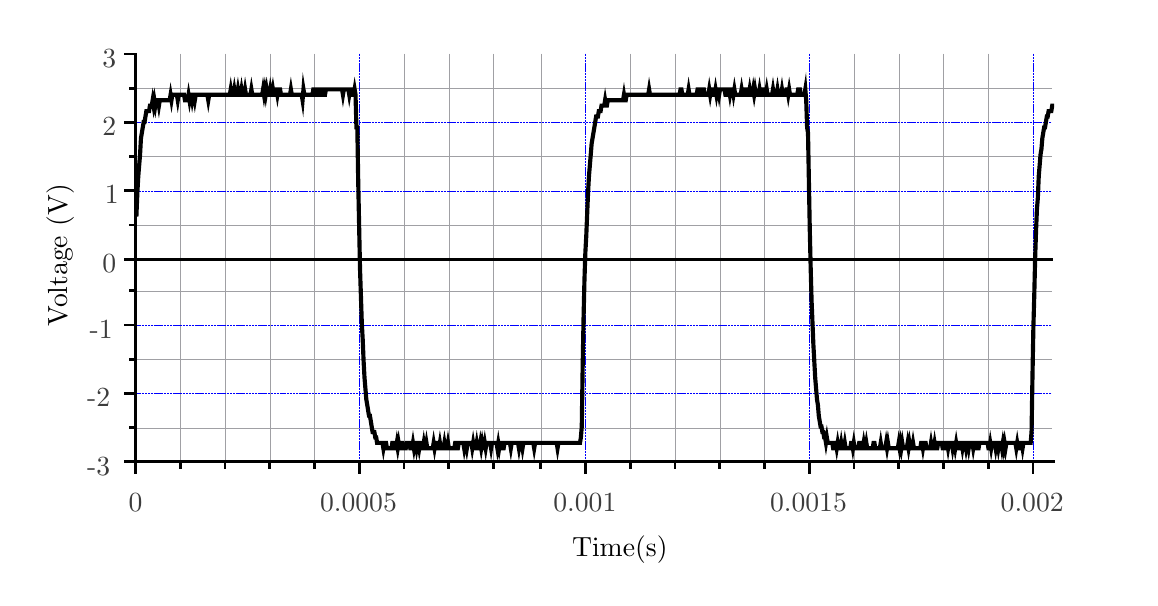
\begin{tikzpicture}{0pt}{0pt}{419pt}{209pt}
	\clip(0pt,209pt) -- (398.436pt,209pt) -- (398.436pt,10.2575pt) -- (0pt,10.2575pt) -- (0pt,209pt);
\begin{scope}
	\clip(38.9878pt,199.491pt) -- (370.859pt,199.491pt) -- (370.859pt,52.098pt) -- (38.9878pt,52.098pt) -- (38.9878pt,199.491pt);
	\color[rgb]{0.627451,0.627451,0.643137}
	\draw[line width=0.1pt, dash pattern=on 0.0024cm off 0.008cm, dash phase=0pt, line join=bevel, line cap=rect](55.1534pt,199.491pt) -- (55.1534pt,53.0489pt);
	\color[rgb]{0.627451,0.627451,0.643137}
	\draw[line width=0.1pt, dash pattern=on 0.0024cm off 0.008cm, dash phase=0pt, line join=bevel, line cap=rect](71.3191pt,199.491pt) -- (71.3191pt,53.0489pt);
	\draw[line width=0.1pt, dash pattern=on 0.0024cm off 0.008cm, dash phase=0pt, line join=bevel, line cap=rect](87.4847pt,199.491pt) -- (87.4847pt,53.0489pt);
	\draw[line width=0.1pt, dash pattern=on 0.0024cm off 0.008cm, dash phase=0pt, line join=bevel, line cap=rect](103.65pt,199.491pt) -- (103.65pt,53.0489pt);
	\draw[line width=0.1pt, dash pattern=on 0.0024cm off 0.008cm, dash phase=0pt, line join=bevel, line cap=rect](135.982pt,199.491pt) -- (135.982pt,53.0489pt);
	\draw[line width=0.1pt, dash pattern=on 0.0024cm off 0.008cm, dash phase=0pt, line join=bevel, line cap=rect](152.147pt,199.491pt) -- (152.147pt,53.0489pt);
	\draw[line width=0.1pt, dash pattern=on 0.0024cm off 0.008cm, dash phase=0pt, line join=bevel, line cap=rect](168.313pt,199.491pt) -- (168.313pt,53.0489pt);
	\draw[line width=0.1pt, dash pattern=on 0.0024cm off 0.008cm, dash phase=0pt, line join=bevel, line cap=rect](185.43pt,199.491pt) -- (185.43pt,53.0489pt);
	\draw[line width=0.1pt, dash pattern=on 0.0024cm off 0.008cm, dash phase=0pt, line join=bevel, line cap=rect](217.761pt,199.491pt) -- (217.761pt,53.0489pt);
	\draw[line width=0.1pt, dash pattern=on 0.0024cm off 0.008cm, dash phase=0pt, line join=bevel, line cap=rect](233.927pt,199.491pt) -- (233.927pt,53.0489pt);
	\draw[line width=0.1pt, dash pattern=on 0.0024cm off 0.008cm, dash phase=0pt, line join=bevel, line cap=rect](250.092pt,199.491pt) -- (250.092pt,53.0489pt);
	\draw[line width=0.1pt, dash pattern=on 0.0024cm off 0.008cm, dash phase=0pt, line join=bevel, line cap=rect](266.258pt,199.491pt) -- (266.258pt,53.0489pt);
	\draw[line width=0.1pt, dash pattern=on 0.0024cm off 0.008cm, dash phase=0pt, line join=bevel, line cap=rect](298.589pt,199.491pt) -- (298.589pt,53.0489pt);
	\draw[line width=0.1pt, dash pattern=on 0.0024cm off 0.008cm, dash phase=0pt, line join=bevel, line cap=rect](314.755pt,199.491pt) -- (314.755pt,53.0489pt);
	\draw[line width=0.1pt, dash pattern=on 0.0024cm off 0.008cm, dash phase=0pt, line join=bevel, line cap=rect](330.921pt,199.491pt) -- (330.921pt,53.0489pt);
	\draw[line width=0.1pt, dash pattern=on 0.0024cm off 0.008cm, dash phase=0pt, line join=bevel, line cap=rect](347.086pt,199.491pt) -- (347.086pt,53.0489pt);
	\draw[line width=0.1pt, dash pattern=on 0.0024cm off 0.008cm, dash phase=0pt, line join=bevel, line cap=rect](38.9878pt,64.46pt) -- (369.908pt,64.46pt);
	\draw[line width=0.1pt, dash pattern=on 0.0024cm off 0.008cm, dash phase=0pt, line join=bevel, line cap=rect](38.9878pt,89.1839pt) -- (369.908pt,89.1839pt);
	\draw[line width=0.1pt, dash pattern=on 0.0024cm off 0.008cm, dash phase=0pt, line join=bevel, line cap=rect](38.9878pt,113.908pt) -- (369.908pt,113.908pt);
	\draw[line width=0.1pt, dash pattern=on 0.0024cm off 0.008cm, dash phase=0pt, line join=bevel, line cap=rect](38.9878pt,137.681pt) -- (369.908pt,137.681pt);
	\draw[line width=0.1pt, dash pattern=on 0.0024cm off 0.008cm, dash phase=0pt, line join=bevel, line cap=rect](38.9878pt,162.405pt) -- (369.908pt,162.405pt);
	\draw[line width=0.1pt, dash pattern=on 0.0024cm off 0.008cm, dash phase=0pt, line join=bevel, line cap=rect](38.9878pt,187.129pt) -- (369.908pt,187.129pt);
	\color[rgb]{0,0,1}
	\draw[line width=0.2pt, dash pattern=on 0.024cm off 0.016cm, dash phase=0pt, line join=bevel, line cap=rect](119.816pt,199.491pt) -- (119.816pt,53.0489pt);
	\draw[line width=0.2pt, dash pattern=on 0.024cm off 0.016cm, dash phase=0pt, line join=bevel, line cap=rect](201.595pt,199.491pt) -- (201.595pt,53.0489pt);
	\draw[line width=0.2pt, dash pattern=on 0.024cm off 0.016cm, dash phase=0pt, line join=bevel, line cap=rect](282.424pt,199.491pt) -- (282.424pt,53.0489pt);
	\draw[line width=0.2pt, dash pattern=on 0.024cm off 0.016cm, dash phase=0pt, line join=bevel, line cap=rect](363.252pt,199.491pt) -- (363.252pt,53.0489pt);
	\draw[line width=0.2pt, dash pattern=on 0.024cm off 0.016cm, dash phase=0pt, line join=bevel, line cap=rect](38.9878pt,76.822pt) -- (369.908pt,76.822pt);
	\draw[line width=0.2pt, dash pattern=on 0.024cm off 0.016cm, dash phase=0pt, line join=bevel, line cap=rect](38.9878pt,101.546pt) -- (369.908pt,101.546pt);
	\draw[line width=0.2pt, dash pattern=on 0.024cm off 0.016cm, dash phase=0pt, line join=bevel, line cap=rect](38.9878pt,125.319pt) -- (369.908pt,125.319pt);
	\draw[line width=0.2pt, dash pattern=on 0.024cm off 0.016cm, dash phase=0pt, line join=bevel, line cap=rect](38.9878pt,150.043pt) -- (369.908pt,150.043pt);
	\draw[line width=0.2pt, dash pattern=on 0.024cm off 0.016cm, dash phase=0pt, line join=bevel, line cap=rect](38.9878pt,174.767pt) -- (369.908pt,174.767pt);
	\color[rgb]{0,0,0}
	\draw[line width=1.5pt, line join=miter, line cap=rect](39.3122pt,141.516pt) -- (39.6366pt,149.377pt) -- (39.961pt,155.273pt) -- (40.2854pt,159.203pt) -- (40.6098pt,163.134pt) -- (40.9342pt,169.03pt) -- (41.2586pt,170.995pt) -- (41.583pt,172.96pt) -- (41.9075pt,174.925pt) -- (42.2319pt,174.925pt) -- (42.5563pt,176.891pt) -- (42.8807pt,178.856pt) -- (43.2051pt,178.856pt) -- (43.5295pt,178.856pt) -- (43.8539pt,178.856pt) -- (44.1783pt,180.821pt) -- (44.5027pt,180.821pt) -- (44.8271pt,180.821pt) -- (45.1516pt,182.786pt) -- (45.476pt,180.821pt) -- (45.8004pt,182.786pt) -- (46.1248pt,180.821pt) -- (46.4492pt,182.786pt) -- (46.7736pt,182.786pt) -- (47.098pt,182.786pt) -- (47.4224pt,180.821pt) -- (47.7468pt,182.786pt) -- (48.0712pt,182.786pt) -- (48.3957pt,182.786pt) -- (48.7201pt,182.786pt) -- (49.0445pt,182.786pt) -- (49.3689pt,182.786pt) -- (49.6933pt,182.786pt) -- (50.0177pt,182.786pt) -- (50.3421pt,182.786pt) -- (50.6665pt,182.786pt) -- (50.9909pt,182.786pt) -- (51.3153pt,182.786pt) -- (51.6398pt,184.752pt) -- (51.9642pt,182.786pt) -- (52.2886pt,184.752pt) -- (52.613pt,184.752pt) -- (52.9374pt,184.752pt) -- (53.2618pt,184.752pt) -- (53.5862pt,184.752pt) -- (53.9106pt,184.752pt) -- (54.235pt,182.786pt) -- (54.5594pt,184.752pt) -- (54.8839pt,184.752pt) -- (55.2083pt,184.752pt) -- (55.5327pt,184.752pt) -- (55.8571pt,184.752pt) -- (56.1815pt,184.752pt) -- (56.5059pt,184.752pt) -- (56.8303pt,182.786pt) -- (57.1547pt,182.786pt) -- (57.4791pt,182.786pt) -- (57.8035pt,182.786pt) -- (58.128pt,184.752pt) -- (58.4524pt,182.786pt) -- (58.7768pt,184.752pt) -- (59.1012pt,184.752pt) -- (59.4256pt,182.786pt) -- (59.75pt,184.752pt) -- (60.0744pt,184.752pt) -- (60.3988pt,182.786pt) -- (60.7232pt,184.752pt) -- (61.0476pt,184.752pt) -- (61.3721pt,184.752pt) -- (61.6965pt,184.752pt) -- (62.0209pt,184.752pt) -- (62.3453pt,184.752pt) -- (62.6697pt,184.752pt) -- (62.9941pt,184.752pt) -- (63.3185pt,184.752pt) -- (63.6429pt,184.752pt) -- (63.9673pt,184.752pt) -- (64.2917pt,184.752pt) -- (64.6162pt,184.752pt) -- (64.9406pt,184.752pt) -- (65.265pt,182.786pt) -- (65.5894pt,184.752pt) -- (65.9138pt,184.752pt) -- (66.2382pt,184.752pt) -- (66.5626pt,184.752pt) -- (66.887pt,184.752pt) -- (67.2114pt,184.752pt) -- (67.5358pt,184.752pt) -- (67.8603pt,184.752pt) -- (68.1847pt,184.752pt) -- (68.5091pt,184.752pt) -- (68.8335pt,184.752pt) -- (69.1579pt,184.752pt) -- (69.4823pt,184.752pt) -- (69.8067pt,184.752pt) -- (70.1311pt,184.752pt) -- (70.4555pt,184.752pt) -- (70.7799pt,184.752pt) -- (71.1044pt,184.752pt) -- (71.4288pt,184.752pt) -- (71.7532pt,184.752pt) -- (72.0776pt,184.752pt) -- (72.402pt,184.752pt) -- (72.7264pt,184.752pt) -- (73.0508pt,184.752pt) -- (73.3752pt,186.717pt) -- (73.6996pt,184.752pt) -- (74.024pt,184.752pt) -- (74.3485pt,184.752pt) -- (74.6729pt,186.717pt) -- (74.9973pt,184.752pt) -- (75.3217pt,184.752pt) -- (75.6461pt,184.752pt) -- (75.9705pt,186.717pt) -- (76.2949pt,184.752pt) -- (76.6193pt,184.752pt) -- (76.9437pt,184.752pt) -- (77.2681pt,186.717pt) -- (77.5926pt,184.752pt) -- (77.917pt,184.752pt) -- (78.2414pt,184.752pt) -- (78.5658pt,186.717pt) -- (78.8902pt,184.752pt) -- (79.2146pt,184.752pt) -- (79.539pt,184.752pt) -- (79.8634pt,184.752pt) -- (80.1878pt,184.752pt) -- (80.5122pt,184.752pt) -- (80.8367pt,186.717pt) -- (81.1611pt,184.752pt) -- (81.4855pt,184.752pt) -- (81.8099pt,184.752pt) -- (82.1343pt,184.752pt) -- (82.4587pt,184.752pt) -- (82.7831pt,184.752pt) -- (83.1075pt,184.752pt) -- (83.4319pt,184.752pt) -- (83.7563pt,184.752pt) -- (84.0808pt,184.752pt) -- (84.4052pt,184.752pt) -- (84.7296pt,184.752pt) -- (85.054pt,186.717pt) -- (85.3784pt,184.752pt) -- (85.7028pt,186.717pt) -- (86.0272pt,184.752pt) -- (86.3516pt,186.717pt) -- (86.676pt,184.752pt) -- (87.0004pt,184.752pt) -- (87.3249pt,184.752pt) -- (87.6493pt,186.717pt) -- (87.9737pt,184.752pt) -- (88.2981pt,184.752pt) -- (88.6225pt,186.717pt) -- (88.9469pt,184.752pt) -- (89.2713pt,184.752pt) -- (89.5957pt,186.717pt) -- (89.9201pt,186.717pt) -- (90.2445pt,184.752pt) -- (90.569pt,186.717pt) -- (90.8934pt,186.717pt) -- (91.2178pt,186.717pt) -- (91.5422pt,184.752pt) -- (91.8666pt,184.752pt) -- (92.191pt,184.752pt) -- (92.5154pt,184.752pt) -- (92.8398pt,184.752pt) -- (93.1642pt,184.752pt) -- (93.4886pt,184.752pt) -- (93.8131pt,184.752pt) -- (94.1375pt,184.752pt) -- (94.4619pt,184.752pt) -- (94.7863pt,184.752pt) -- (95.1107pt,186.717pt) -- (95.4351pt,184.752pt) -- (95.7595pt,184.752pt) -- (96.0839pt,184.752pt) -- (96.4083pt,184.752pt) -- (96.7327pt,184.752pt) -- (97.0572pt,184.752pt) -- (97.3816pt,184.752pt) -- (97.706pt,184.752pt) -- (98.0304pt,184.752pt) -- (98.3548pt,184.752pt) -- (98.6792pt,184.752pt) -- (99.0036pt,184.752pt) -- (99.328pt,182.786pt) -- (99.6524pt,186.717pt) -- (99.9768pt,184.752pt) -- (100.301pt,184.752pt) -- (100.626pt,184.752pt) -- (100.95pt,184.752pt) -- (101.274pt,184.752pt) -- (101.599pt,184.752pt) -- (101.923pt,184.752pt) -- (102.248pt,184.752pt) -- (102.572pt,184.752pt) -- (102.897pt,184.752pt) -- (103.221pt,186.717pt) -- (103.545pt,186.717pt) -- (103.87pt,184.752pt) -- (104.194pt,184.752pt) -- (104.519pt,184.752pt) -- (104.843pt,186.717pt) -- (105.167pt,186.717pt) -- (105.492pt,184.752pt) -- (105.816pt,184.752pt) -- (106.141pt,186.717pt) -- (106.465pt,186.717pt) -- (106.789pt,186.717pt) -- (107.114pt,184.752pt) -- (107.438pt,184.752pt) -- (107.763pt,186.717pt) -- (108.087pt,186.717pt) -- (108.412pt,186.717pt) -- (108.736pt,186.717pt) -- (109.06pt,186.717pt) -- (109.385pt,186.717pt) -- (109.709pt,186.717pt) -- (110.034pt,186.717pt) -- (110.358pt,186.717pt) -- (110.682pt,186.717pt) -- (111.007pt,186.717pt) -- (111.331pt,186.717pt) -- (111.656pt,186.717pt) -- (111.98pt,186.717pt) -- (112.304pt,186.717pt) -- (112.629pt,186.717pt) -- (112.953pt,186.717pt) -- (113.278pt,186.717pt) -- (113.602pt,186.717pt) -- (113.926pt,184.752pt) -- (114.251pt,186.717pt) -- (114.575pt,186.717pt) -- (114.9pt,186.717pt) -- (115.224pt,186.717pt) -- (115.549pt,186.717pt) -- (115.873pt,186.717pt) -- (116.197pt,184.752pt) -- (116.522pt,186.717pt) -- (116.846pt,186.717pt) -- (117.171pt,186.717pt) -- (117.495pt,184.752pt) -- (117.819pt,184.752pt) -- (118.144pt,186.717pt) -- (118.468pt,184.752pt) -- (118.793pt,172.96pt) -- (119.117pt,172.96pt) -- (119.441pt,153.308pt) -- (119.766pt,137.586pt) -- (120.09pt,121.864pt) -- (120.415pt,112.038pt) -- (120.739pt,102.212pt) -- (121.063pt,96.3159pt) -- (121.388pt,88.4549pt) -- (121.712pt,82.5592pt) -- (122.037pt,78.6287pt) -- (122.361pt,74.6982pt) -- (122.686pt,72.733pt) -- (123.01pt,70.7678pt) -- (123.334pt,68.8025pt) -- (123.659pt,68.8025pt) -- (123.983pt,66.8373pt) -- (124.308pt,64.8721pt) -- (124.632pt,62.9068pt) -- (124.956pt,62.9068pt) -- (125.281pt,62.9068pt) -- (125.605pt,60.9416pt) -- (125.93pt,60.9416pt) -- (126.254pt,58.9764pt) -- (126.578pt,58.9764pt) -- (126.903pt,58.9764pt) -- (127.227pt,58.9764pt) -- (127.552pt,58.9764pt) -- (127.876pt,58.9764pt) -- (128.201pt,58.9764pt) -- (128.525pt,57.0111pt) -- (128.849pt,58.9764pt) -- (129.174pt,58.9764pt) -- (129.498pt,58.9764pt) -- (129.823pt,57.0111pt) -- (130.147pt,57.0111pt) -- (130.471pt,57.0111pt) -- (130.796pt,57.0111pt) -- (131.12pt,57.0111pt) -- (131.445pt,57.0111pt) -- (131.769pt,58.9764pt) -- (132.093pt,58.9764pt) -- (132.418pt,57.0111pt) -- (132.742pt,57.0111pt) -- (133.067pt,57.0111pt) -- (133.391pt,58.9764pt) -- (133.715pt,57.0111pt) -- (134.04pt,58.9764pt) -- (134.364pt,57.0111pt) -- (134.689pt,57.0111pt) -- (135.013pt,58.9764pt) -- (135.338pt,58.9764pt) -- (135.662pt,57.0111pt) -- (135.986pt,57.0111pt) -- (136.311pt,57.0111pt) -- (136.635pt,57.0111pt) -- (136.96pt,58.9764pt) -- (137.284pt,58.9764pt) -- (137.608pt,58.9764pt) -- (137.933pt,58.9764pt) -- (138.257pt,57.0111pt) -- (138.582pt,57.0111pt) -- (138.906pt,57.0111pt) -- (139.23pt,58.9764pt) -- (139.555pt,57.0111pt) -- (139.879pt,58.9764pt) -- (140.204pt,58.9764pt) -- (140.528pt,57.0111pt) -- (140.853pt,58.9764pt) -- (141.177pt,58.9764pt) -- (141.501pt,57.0111pt) -- (141.826pt,58.9764pt) -- (142.15pt,58.9764pt) -- (142.475pt,57.0111pt) -- (142.799pt,57.0111pt) -- (143.123pt,58.9764pt) -- (143.448pt,57.0111pt) -- (143.772pt,57.0111pt) -- (144.097pt,58.9764pt) -- (144.421pt,57.0111pt) -- (144.745pt,57.0111pt) -- (145.07pt,57.0111pt) -- (145.394pt,57.0111pt) -- (145.719pt,57.0111pt) -- (146.043pt,57.0111pt) -- (146.367pt,57.0111pt) -- (146.692pt,58.9764pt) -- (147.016pt,57.0111pt) -- (147.341pt,58.9764pt) -- (147.665pt,58.9764pt) -- (147.99pt,57.0111pt) -- (148.314pt,57.0111pt) -- (148.638pt,57.0111pt) -- (148.963pt,58.9764pt) -- (149.287pt,57.0111pt) -- (149.612pt,57.0111pt) -- (149.936pt,57.0111pt) -- (150.26pt,57.0111pt) -- (150.585pt,58.9764pt) -- (150.909pt,57.0111pt) -- (151.234pt,57.0111pt) -- (151.558pt,57.0111pt) -- (151.882pt,58.9764pt) -- (152.207pt,57.0111pt) -- (152.531pt,57.0111pt) -- (152.856pt,57.0111pt) -- (153.18pt,57.0111pt) -- (153.504pt,57.0111pt) -- (153.829pt,57.0111pt) -- (154.153pt,57.0111pt) -- (154.478pt,58.9764pt) -- (154.802pt,58.9764pt) -- (155.127pt,57.0111pt) -- (155.451pt,57.0111pt) -- (155.775pt,58.9764pt) -- (156.1pt,58.9764pt) -- (156.424pt,58.9764pt) -- (156.749pt,58.9764pt) -- (157.073pt,58.9764pt) -- (157.397pt,58.9764pt) -- (157.722pt,57.0111pt) -- (158.046pt,58.9764pt) -- (158.371pt,58.9764pt) -- (158.695pt,57.0111pt) -- (159.019pt,58.9764pt) -- (159.344pt,58.9764pt) -- (159.668pt,58.9764pt) -- (159.993pt,58.9764pt) -- (160.317pt,58.9764pt) -- (160.642pt,57.0111pt) -- (160.966pt,58.9764pt) -- (161.29pt,57.0111pt) -- (161.615pt,57.0111pt) -- (161.939pt,57.0111pt) -- (162.264pt,58.9764pt) -- (162.588pt,57.0111pt) -- (162.912pt,57.0111pt) -- (163.237pt,57.0111pt) -- (163.561pt,58.9764pt) -- (163.886pt,57.0111pt) -- (164.21pt,58.9764pt) -- (164.534pt,57.0111pt) -- (164.859pt,57.0111pt) -- (165.183pt,58.9764pt) -- (165.508pt,57.0111pt) -- (165.832pt,58.9764pt) -- (166.156pt,58.9764pt) -- (166.481pt,58.9764pt) -- (166.805pt,58.9764pt) -- (167.13pt,58.9764pt) -- (167.454pt,57.0111pt) -- (167.779pt,58.9764pt) -- (168.103pt,58.9764pt) -- (168.427pt,58.9764pt) -- (168.752pt,58.9764pt) -- (169.076pt,58.9764pt) -- (169.401pt,58.9764pt) -- (169.725pt,57.0111pt) -- (170.049pt,58.9764pt) -- (170.374pt,57.0111pt) -- (170.698pt,58.9764pt) -- (171.023pt,58.9764pt) -- (171.347pt,58.9764pt) -- (171.671pt,57.0111pt) -- (171.996pt,57.0111pt) -- (172.32pt,58.9764pt) -- (172.645pt,58.9764pt) -- (172.969pt,58.9764pt) -- (173.294pt,58.9764pt) -- (173.618pt,58.9764pt) -- (173.942pt,58.9764pt) -- (174.267pt,58.9764pt) -- (174.591pt,57.0111pt) -- (174.916pt,58.9764pt) -- (175.24pt,58.9764pt) -- (175.564pt,58.9764pt) -- (175.889pt,58.9764pt) -- (176.213pt,58.9764pt) -- (176.538pt,58.9764pt) -- (176.862pt,58.9764pt) -- (177.186pt,58.9764pt) -- (177.511pt,57.0111pt) -- (177.835pt,58.9764pt) -- (178.16pt,58.9764pt) -- (178.484pt,58.9764pt) -- (178.808pt,57.0111pt) -- (179.133pt,58.9764pt) -- (179.457pt,58.9764pt) -- (179.782pt,58.9764pt) -- (180.106pt,58.9764pt) -- (180.431pt,58.9764pt) -- (180.755pt,58.9764pt) -- (181.079pt,58.9764pt) -- (181.404pt,58.9764pt) -- (181.728pt,58.9764pt) -- (182.053pt,58.9764pt) -- (182.377pt,58.9764pt) -- (182.701pt,58.9764pt) -- (183.026pt,57.0111pt) -- (183.35pt,58.9764pt) -- (183.675pt,58.9764pt) -- (183.999pt,58.9764pt) -- (184.323pt,58.9764pt) -- (184.648pt,58.9764pt) -- (184.972pt,58.9764pt) -- (185.297pt,58.9764pt) -- (185.621pt,58.9764pt) -- (185.946pt,58.9764pt) -- (186.27pt,58.9764pt) -- (186.594pt,58.9764pt) -- (186.919pt,58.9764pt) -- (187.243pt,58.9764pt) -- (187.568pt,58.9764pt) -- (187.892pt,58.9764pt) -- (188.216pt,58.9764pt) -- (188.541pt,58.9764pt) -- (188.865pt,58.9764pt) -- (189.19pt,58.9764pt) -- (189.514pt,58.9764pt) -- (189.838pt,58.9764pt) -- (190.163pt,58.9764pt) -- (190.487pt,58.9764pt) -- (190.812pt,58.9764pt) -- (191.136pt,58.9764pt) -- (191.46pt,57.0111pt) -- (191.785pt,58.9764pt) -- (192.109pt,58.9764pt) -- (192.434pt,58.9764pt) -- (192.758pt,58.9764pt) -- (193.083pt,58.9764pt) -- (193.407pt,58.9764pt) -- (193.731pt,58.9764pt) -- (194.056pt,58.9764pt) -- (194.38pt,58.9764pt) -- (194.705pt,58.9764pt) -- (195.029pt,58.9764pt) -- (195.353pt,58.9764pt) -- (195.678pt,58.9764pt) -- (196.002pt,58.9764pt) -- (196.327pt,58.9764pt) -- (196.651pt,58.9764pt) -- (196.975pt,58.9764pt) -- (197.3pt,58.9764pt) -- (197.624pt,58.9764pt) -- (197.949pt,58.9764pt) -- (198.273pt,58.9764pt) -- (198.597pt,58.9764pt) -- (198.922pt,58.9764pt) -- (199.246pt,58.9764pt) -- (199.571pt,58.9764pt) -- (199.895pt,60.9416pt) -- (200.22pt,64.8721pt) -- (200.544pt,86.4897pt) -- (200.868pt,104.177pt) -- (201.193pt,117.933pt) -- (201.517pt,127.76pt) -- (201.842pt,133.655pt) -- (202.166pt,141.516pt) -- (202.49pt,149.377pt) -- (202.815pt,155.273pt) -- (203.139pt,159.203pt) -- (203.464pt,163.134pt) -- (203.788pt,167.064pt) -- (204.112pt,169.03pt) -- (204.437pt,170.995pt) -- (204.761pt,172.96pt) -- (205.086pt,174.925pt) -- (205.41pt,176.891pt) -- (205.735pt,176.891pt) -- (206.059pt,176.891pt) -- (206.383pt,178.856pt) -- (206.708pt,178.856pt) -- (207.032pt,178.856pt) -- (207.357pt,180.821pt) -- (207.681pt,180.821pt) -- (208.005pt,180.821pt) -- (208.33pt,180.821pt) -- (208.654pt,182.786pt) -- (208.979pt,180.821pt) -- (209.303pt,180.821pt) -- (209.627pt,182.786pt) -- (209.952pt,182.786pt) -- (210.276pt,182.786pt) -- (210.601pt,182.786pt) -- (210.925pt,182.786pt) -- (211.249pt,182.786pt) -- (211.574pt,182.786pt) -- (211.898pt,182.786pt) -- (212.223pt,182.786pt) -- (212.547pt,182.786pt) -- (212.872pt,182.786pt) -- (213.196pt,182.786pt) -- (213.52pt,182.786pt) -- (213.845pt,182.786pt) -- (214.169pt,182.786pt) -- (214.494pt,182.786pt) -- (214.818pt,182.786pt) -- (215.142pt,182.786pt) -- (215.467pt,184.752pt) -- (215.791pt,182.786pt) -- (216.116pt,182.786pt) -- (216.44pt,184.752pt) -- (216.764pt,184.752pt) -- (217.089pt,184.752pt) -- (217.413pt,184.752pt) -- (217.738pt,184.752pt) -- (218.062pt,184.752pt) -- (218.387pt,184.752pt) -- (218.711pt,184.752pt) -- (219.035pt,184.752pt) -- (219.36pt,184.752pt) -- (219.684pt,184.752pt) -- (220.009pt,184.752pt) -- (220.333pt,184.752pt) -- (220.657pt,184.752pt) -- (220.982pt,184.752pt) -- (221.306pt,184.752pt) -- (221.631pt,184.752pt) -- (221.955pt,184.752pt) -- (222.279pt,184.752pt) -- (222.604pt,184.752pt) -- (222.928pt,184.752pt) -- (223.253pt,184.752pt) -- (223.577pt,184.752pt) -- (223.901pt,184.752pt) -- (224.226pt,184.752pt) -- (224.55pt,186.717pt) -- (224.875pt,184.752pt) -- (225.199pt,184.752pt) -- (225.524pt,184.752pt) -- (225.848pt,184.752pt) -- (226.172pt,184.752pt) -- (226.497pt,184.752pt) -- (226.821pt,184.752pt) -- (227.146pt,184.752pt) -- (227.47pt,184.752pt) -- (227.794pt,184.752pt) -- (228.119pt,184.752pt) -- (228.443pt,184.752pt) -- (228.768pt,184.752pt) -- (229.092pt,184.752pt) -- (229.416pt,184.752pt) -- (229.741pt,184.752pt) -- (230.065pt,184.752pt) -- (230.39pt,184.752pt) -- (230.714pt,184.752pt) -- (231.038pt,184.752pt) -- (231.363pt,184.752pt) -- (231.687pt,184.752pt) -- (232.012pt,184.752pt) -- (232.336pt,184.752pt) -- (232.661pt,184.752pt) -- (232.985pt,184.752pt) -- (233.309pt,184.752pt) -- (233.634pt,184.752pt) -- (233.958pt,184.752pt) -- (234.283pt,184.752pt) -- (234.607pt,184.752pt) -- (234.931pt,184.752pt) -- (235.256pt,184.752pt) -- (235.58pt,184.752pt) -- (235.905pt,186.717pt) -- (236.229pt,186.717pt) -- (236.553pt,184.752pt) -- (236.878pt,184.752pt) -- (237.202pt,184.752pt) -- (237.527pt,184.752pt) -- (237.851pt,184.752pt) -- (238.176pt,184.752pt) -- (238.5pt,184.752pt) -- (238.824pt,186.717pt) -- (239.149pt,184.752pt) -- (239.473pt,184.752pt) -- (239.798pt,184.752pt) -- (240.122pt,184.752pt) -- (240.446pt,184.752pt) -- (240.771pt,184.752pt) -- (241.095pt,184.752pt) -- (241.42pt,184.752pt) -- (241.744pt,184.752pt) -- (242.068pt,186.717pt) -- (242.393pt,186.717pt) -- (242.717pt,184.752pt) -- (243.042pt,184.752pt) -- (243.366pt,184.752pt) -- (243.69pt,186.717pt) -- (244.015pt,186.717pt) -- (244.339pt,186.717pt) -- (244.664pt,184.752pt) -- (244.988pt,184.752pt) -- (245.313pt,184.752pt) -- (245.637pt,184.752pt) -- (245.961pt,184.752pt) -- (246.286pt,186.717pt) -- (246.61pt,184.752pt) -- (246.935pt,186.717pt) -- (247.259pt,186.717pt) -- (247.583pt,186.717pt) -- (247.908pt,184.752pt) -- (248.232pt,184.752pt) -- (248.557pt,186.717pt) -- (248.881pt,184.752pt) -- (249.205pt,186.717pt) -- (249.53pt,186.717pt) -- (249.854pt,184.752pt) -- (250.179pt,186.717pt) -- (250.503pt,186.717pt) -- (250.828pt,186.717pt) -- (251.152pt,186.717pt) -- (251.476pt,186.717pt) -- (251.801pt,186.717pt) -- (252.125pt,184.752pt) -- (252.45pt,184.752pt) -- (252.774pt,186.717pt) -- (253.098pt,186.717pt) -- (253.423pt,186.717pt) -- (253.747pt,184.752pt) -- (254.072pt,186.717pt) -- (254.396pt,186.717pt) -- (254.72pt,186.717pt) -- (255.045pt,184.752pt) -- (255.369pt,186.717pt) -- (255.694pt,184.752pt) -- (256.018pt,184.752pt) -- (256.342pt,184.752pt) -- (256.667pt,184.752pt) -- (256.991pt,184.752pt) -- (257.316pt,184.752pt) -- (257.64pt,184.752pt) -- (257.965pt,186.717pt) -- (258.289pt,184.752pt) -- (258.613pt,184.752pt) -- (258.938pt,186.717pt) -- (259.262pt,186.717pt) -- (259.587pt,186.717pt) -- (259.911pt,184.752pt) -- (260.235pt,184.752pt) -- (260.56pt,184.752pt) -- (260.884pt,186.717pt) -- (261.209pt,184.752pt) -- (261.533pt,184.752pt) -- (261.857pt,184.752pt) -- (262.182pt,186.717pt) -- (262.506pt,184.752pt) -- (262.831pt,186.717pt) -- (263.155pt,184.752pt) -- (263.479pt,184.752pt) -- (263.804pt,184.752pt) -- (264.128pt,184.752pt) -- (264.453pt,186.717pt) -- (264.777pt,184.752pt) -- (265.102pt,184.752pt) -- (265.426pt,186.717pt) -- (265.75pt,186.717pt) -- (266.075pt,184.752pt) -- (266.399pt,184.752pt) -- (266.724pt,184.752pt) -- (267.048pt,186.717pt) -- (267.372pt,184.752pt) -- (267.697pt,184.752pt) -- (268.021pt,184.752pt) -- (268.346pt,184.752pt) -- (268.67pt,184.752pt) -- (268.994pt,184.752pt) -- (269.319pt,186.717pt) -- (269.643pt,184.752pt) -- (269.968pt,184.752pt) -- (270.292pt,184.752pt) -- (270.617pt,184.752pt) -- (270.941pt,186.717pt) -- (271.265pt,184.752pt) -- (271.59pt,184.752pt) -- (271.914pt,184.752pt) -- (272.239pt,184.752pt) -- (272.563pt,186.717pt) -- (272.887pt,184.752pt) -- (273.212pt,184.752pt) -- (273.536pt,184.752pt) -- (273.861pt,184.752pt) -- (274.185pt,186.717pt) -- (274.509pt,186.717pt) -- (274.834pt,184.752pt) -- (275.158pt,186.717pt) -- (275.483pt,184.752pt) -- (275.807pt,184.752pt) -- (276.131pt,184.752pt) -- (276.456pt,184.752pt) -- (276.78pt,184.752pt) -- (277.105pt,184.752pt) -- (277.429pt,184.752pt) -- (277.754pt,184.752pt) -- (278.078pt,184.752pt) -- (278.402pt,186.717pt) -- (278.727pt,186.717pt) -- (279.051pt,186.717pt) -- (279.376pt,184.752pt) -- (279.7pt,184.752pt) -- (280.024pt,184.752pt) -- (280.349pt,184.752pt) -- (280.673pt,184.752pt) -- (280.998pt,186.717pt) -- (281.322pt,182.786pt) -- (281.646pt,172.96pt) -- (281.971pt,170.995pt) -- (282.295pt,153.308pt) -- (282.62pt,135.621pt) -- (282.944pt,121.864pt) -- (283.269pt,110.073pt) -- (283.593pt,102.212pt) -- (283.917pt,94.3506pt) -- (284.242pt,88.4549pt) -- (284.566pt,82.5592pt) -- (284.891pt,78.6287pt) -- (285.215pt,74.6982pt) -- (285.539pt,72.733pt) -- (285.864pt,68.8025pt) -- (286.188pt,66.8373pt) -- (286.513pt,64.8721pt) -- (286.837pt,64.8721pt) -- (287.161pt,62.9068pt) -- (287.486pt,62.9068pt) -- (287.81pt,60.9416pt) -- (288.135pt,60.9416pt) -- (288.459pt,58.9764pt) -- (288.783pt,60.9416pt) -- (289.108pt,58.9764pt) -- (289.432pt,58.9764pt) -- (289.757pt,58.9764pt) -- (290.081pt,58.9764pt) -- (290.406pt,58.9764pt) -- (290.73pt,58.9764pt) -- (291.054pt,57.0111pt) -- (291.379pt,57.0111pt) -- (291.703pt,58.9764pt) -- (292.028pt,58.9764pt) -- (292.352pt,57.0111pt) -- (292.676pt,58.9764pt) -- (293.001pt,57.0111pt) -- (293.325pt,57.0111pt) -- (293.65pt,57.0111pt) -- (293.974pt,58.9764pt) -- (294.298pt,57.0111pt) -- (294.623pt,57.0111pt) -- (294.947pt,57.0111pt) -- (295.272pt,58.9764pt) -- (295.596pt,57.0111pt) -- (295.92pt,57.0111pt) -- (296.245pt,57.0111pt) -- (296.569pt,57.0111pt) -- (296.894pt,57.0111pt) -- (297.218pt,57.0111pt) -- (297.543pt,58.9764pt) -- (297.867pt,58.9764pt) -- (298.191pt,57.0111pt) -- (298.516pt,58.9764pt) -- (298.84pt,57.0111pt) -- (299.165pt,57.0111pt) -- (299.489pt,57.0111pt) -- (299.813pt,57.0111pt) -- (300.138pt,57.0111pt) -- (300.462pt,58.9764pt) -- (300.787pt,58.9764pt) -- (301.111pt,57.0111pt) -- (301.435pt,57.0111pt) -- (301.76pt,57.0111pt) -- (302.084pt,58.9764pt) -- (302.409pt,57.0111pt) -- (302.733pt,57.0111pt) -- (303.058pt,58.9764pt) -- (303.382pt,57.0111pt) -- (303.706pt,57.0111pt) -- (304.031pt,57.0111pt) -- (304.355pt,57.0111pt) -- (304.68pt,57.0111pt) -- (305.004pt,57.0111pt) -- (305.328pt,57.0111pt) -- (305.653pt,58.9764pt) -- (305.977pt,58.9764pt) -- (306.302pt,57.0111pt) -- (306.626pt,57.0111pt) -- (306.95pt,57.0111pt) -- (307.275pt,57.0111pt) -- (307.599pt,57.0111pt) -- (307.924pt,57.0111pt) -- (308.248pt,58.9764pt) -- (308.572pt,57.0111pt) -- (308.897pt,57.0111pt) -- (309.221pt,57.0111pt) -- (309.546pt,57.0111pt) -- (309.87pt,57.0111pt) -- (310.195pt,58.9764pt) -- (310.519pt,57.0111pt) -- (310.843pt,58.9764pt) -- (311.168pt,57.0111pt) -- (311.492pt,57.0111pt) -- (311.817pt,57.0111pt) -- (312.141pt,57.0111pt) -- (312.465pt,57.0111pt) -- (312.79pt,57.0111pt) -- (313.114pt,57.0111pt) -- (313.439pt,57.0111pt) -- (313.763pt,57.0111pt) -- (314.087pt,57.0111pt) -- (314.412pt,57.0111pt) -- (314.736pt,58.9764pt) -- (315.061pt,57.0111pt) -- (315.385pt,58.9764pt) -- (315.71pt,57.0111pt) -- (316.034pt,58.9764pt) -- (316.358pt,57.0111pt) -- (316.683pt,57.0111pt) -- (317.007pt,57.0111pt) -- (317.332pt,57.0111pt) -- (317.656pt,57.0111pt) -- (317.98pt,58.9764pt) -- (318.305pt,57.0111pt) -- (318.629pt,58.9764pt) -- (318.954pt,57.0111pt) -- (319.278pt,57.0111pt) -- (319.602pt,57.0111pt) -- (319.927pt,58.9764pt) -- (320.251pt,57.0111pt) -- (320.576pt,57.0111pt) -- (320.9pt,57.0111pt) -- (321.224pt,57.0111pt) -- (321.549pt,57.0111pt) -- (321.873pt,57.0111pt) -- (322.198pt,57.0111pt) -- (322.522pt,57.0111pt) -- (322.847pt,58.9764pt) -- (323.171pt,58.9764pt) -- (323.495pt,57.0111pt) -- (323.82pt,58.9764pt) -- (324.144pt,58.9764pt) -- (324.469pt,58.9764pt) -- (324.793pt,57.0111pt) -- (325.117pt,57.0111pt) -- (325.442pt,57.0111pt) -- (325.766pt,57.0111pt) -- (326.091pt,57.0111pt) -- (326.415pt,58.9764pt) -- (326.739pt,57.0111pt) -- (327.064pt,57.0111pt) -- (327.388pt,57.0111pt) -- (327.713pt,58.9764pt) -- (328.037pt,57.0111pt) -- (328.361pt,57.0111pt) -- (328.686pt,57.0111pt) -- (329.01pt,58.9764pt) -- (329.335pt,58.9764pt) -- (329.659pt,58.9764pt) -- (329.984pt,58.9764pt) -- (330.308pt,58.9764pt) -- (330.632pt,57.0111pt) -- (330.957pt,57.0111pt) -- (331.281pt,57.0111pt) -- (331.606pt,58.9764pt) -- (331.93pt,58.9764pt) -- (332.254pt,58.9764pt) -- (332.579pt,57.0111pt) -- (332.903pt,58.9764pt) -- (333.228pt,58.9764pt) -- (333.552pt,58.9764pt) -- (333.876pt,58.9764pt) -- (334.201pt,57.0111pt) -- (334.525pt,58.9764pt) -- (334.85pt,58.9764pt) -- (335.174pt,57.0111pt) -- (335.499pt,58.9764pt) -- (335.823pt,57.0111pt) -- (336.147pt,57.0111pt) -- (336.472pt,57.0111pt) -- (336.796pt,58.9764pt) -- (337.121pt,58.9764pt) -- (337.445pt,58.9764pt) -- (337.769pt,57.0111pt) -- (338.094pt,58.9764pt) -- (338.418pt,58.9764pt) -- (338.743pt,58.9764pt) -- (339.067pt,57.0111pt) -- (339.391pt,58.9764pt) -- (339.716pt,58.9764pt) -- (340.04pt,57.0111pt) -- (340.365pt,58.9764pt) -- (340.689pt,58.9764pt) -- (341.013pt,58.9764pt) -- (341.338pt,58.9764pt) -- (341.662pt,57.0111pt) -- (341.987pt,58.9764pt) -- (342.311pt,58.9764pt) -- (342.636pt,58.9764pt) -- (342.96pt,57.0111pt) -- (343.284pt,57.0111pt) -- (343.609pt,57.0111pt) -- (343.933pt,58.9764pt) -- (344.258pt,58.9764pt) -- (344.582pt,58.9764pt) -- (344.906pt,58.9764pt) -- (345.231pt,58.9764pt) -- (345.555pt,58.9764pt) -- (345.88pt,58.9764pt) -- (346.204pt,58.9764pt) -- (346.528pt,58.9764pt) -- (346.853pt,58.9764pt) -- (347.177pt,57.0111pt) -- (347.502pt,57.0111pt) -- (347.826pt,58.9764pt) -- (348.151pt,57.0111pt) -- (348.475pt,58.9764pt) -- (348.799pt,58.9764pt) -- (349.124pt,58.9764pt) -- (349.448pt,58.9764pt) -- (349.773pt,57.0111pt) -- (350.097pt,58.9764pt) -- (350.421pt,58.9764pt) -- (350.746pt,57.0111pt) -- (351.07pt,58.9764pt) -- (351.395pt,58.9764pt) -- (351.719pt,58.9764pt) -- (352.043pt,57.0111pt) -- (352.368pt,58.9764pt) -- (352.692pt,57.0111pt) -- (353.017pt,58.9764pt) -- (353.341pt,57.0111pt) -- (353.665pt,58.9764pt) -- (353.99pt,58.9764pt) -- (354.314pt,58.9764pt) -- (354.639pt,58.9764pt) -- (354.963pt,58.9764pt) -- (355.288pt,58.9764pt) -- (355.612pt,58.9764pt) -- (355.936pt,58.9764pt) -- (356.261pt,58.9764pt) -- (356.585pt,58.9764pt) -- (356.91pt,58.9764pt) -- (357.234pt,57.0111pt) -- (357.558pt,58.9764pt) -- (357.883pt,57.0111pt) -- (358.207pt,57.0111pt) -- (358.532pt,57.0111pt) -- (358.856pt,58.9764pt) -- (359.18pt,58.9764pt) -- (359.505pt,57.0111pt) -- (359.829pt,58.9764pt) -- (360.154pt,58.9764pt) -- (360.478pt,58.9764pt) -- (360.803pt,58.9764pt) -- (361.127pt,58.9764pt) -- (361.451pt,58.9764pt) -- (361.776pt,58.9764pt) -- (362.1pt,58.9764pt) -- (362.425pt,58.9764pt) -- (362.749pt,62.9068pt) -- (363.073pt,82.5592pt) -- (363.398pt,100.246pt) -- (363.722pt,112.038pt) -- (364.047pt,125.794pt) -- (364.371pt,135.621pt) -- (364.695pt,143.482pt) -- (365.02pt,147.412pt) -- (365.344pt,155.273pt) -- (365.669pt,159.203pt) -- (365.993pt,163.134pt) -- (366.317pt,165.099pt) -- (366.642pt,169.03pt) -- (366.966pt,170.995pt) -- (367.291pt,172.96pt) -- (367.615pt,172.96pt) -- (367.94pt,174.925pt) -- (368.264pt,176.891pt) -- (368.588pt,176.891pt) -- (368.913pt,178.856pt) -- (369.237pt,178.856pt) -- (369.562pt,178.856pt) -- (369.886pt,178.856pt) -- (370.21pt,180.821pt) -- (370.535pt,180.821pt) -- (370.859pt,180.821pt);
	\draw[line width=1pt, line join=bevel, line cap=rect](38.9878pt,125.319pt) -- (369.908pt,125.319pt);
\end{scope}
\begin{scope}
	\color[rgb]{0,0,0}
	\pgftext[center, base, at={\pgfpoint{14.2638pt}{126.738pt}},rotate=90]{Voltage (V)}
	\color[rgb]{0.235294,0.235294,0.235294}
	\pgftext[center, base, at={\pgfpoint{25.6154pt}{47.3434pt}}]{-3}
	\pgftext[center, base, at={\pgfpoint{25.6154pt}{72.0674pt}}]{-2}
	\pgftext[center, base, at={\pgfpoint{26.5664pt}{96.7913pt}}]{-1}
	\pgftext[center, base, at={\pgfpoint{29.4488pt}{120.564pt}}]{0}
	\pgftext[center, base, at={\pgfpoint{30.3998pt}{145.288pt}}]{1}
	\pgftext[center, base, at={\pgfpoint{29.4488pt}{170.012pt}}]{2}
	\pgftext[center, base, at={\pgfpoint{29.4488pt}{194.736pt}}]{3}
	\color[rgb]{0,0,0}
	\draw[line width=1pt, line join=bevel, line cap=rect](38.9878pt,64.46pt) -- (37.0859pt,64.46pt);
	\draw[line width=1pt, line join=bevel, line cap=rect](38.9878pt,89.1839pt) -- (37.0859pt,89.1839pt);
	\draw[line width=1pt, line join=bevel, line cap=rect](38.9878pt,113.908pt) -- (37.0859pt,113.908pt);
	\draw[line width=1pt, line join=bevel, line cap=rect](38.9878pt,137.681pt) -- (37.0859pt,137.681pt);
	\draw[line width=1pt, line join=bevel, line cap=rect](38.9878pt,162.405pt) -- (37.0859pt,162.405pt);
	\draw[line width=1pt, line join=bevel, line cap=rect](38.9878pt,187.129pt) -- (37.0859pt,187.129pt);
	\draw[line width=1pt, line join=bevel, line cap=rect](38.9878pt,52.098pt) -- (35.1841pt,52.098pt);
	\draw[line width=1pt, line join=bevel, line cap=rect](38.9878pt,76.822pt) -- (35.1841pt,76.822pt);
	\draw[line width=1pt, line join=bevel, line cap=rect](38.9878pt,101.546pt) -- (35.1841pt,101.546pt);
	\draw[line width=1pt, line join=bevel, line cap=rect](38.9878pt,125.319pt) -- (35.1841pt,125.319pt);
	\draw[line width=1pt, line join=bevel, line cap=rect](38.9878pt,150.043pt) -- (35.1841pt,150.043pt);
	\draw[line width=1pt, line join=bevel, line cap=rect](38.9878pt,174.767pt) -- (35.1841pt,174.767pt);
	\draw[line width=1pt, line join=bevel, line cap=rect](38.9878pt,199.491pt) -- (35.1841pt,199.491pt);
	\draw[line width=1pt, line join=bevel, line cap=rect](38.9878pt,199.491pt) -- (38.9878pt,52.098pt);
	\pgftext[center, base, at={\pgfpoint{213.957pt}{17.8649pt}}]{Time(s)}
	\color[rgb]{0.235294,0.235294,0.235294}
	\pgftext[center, base, at={\pgfpoint{38.958pt}{34.0305pt}}]{0}
	\pgftext[center, base, at={\pgfpoint{119.534pt}{34.0305pt}}]{0.0005}
	\pgftext[center, base, at={\pgfpoint{201.343pt}{34.0305pt}}]{0.001}
	\pgftext[center, base, at={\pgfpoint{282.141pt}{34.0305pt}}]{0.0015}
	\pgftext[center, base, at={\pgfpoint{362.999pt}{34.0305pt}}]{0.002}
	\color[rgb]{0,0,0}
	\draw[line width=1pt, line join=bevel, line cap=rect](55.1534pt,52.098pt) -- (55.1534pt,50.1962pt);
	\draw[line width=1pt, line join=bevel, line cap=rect](71.3191pt,52.098pt) -- (71.3191pt,50.1962pt);
	\draw[line width=1pt, line join=bevel, line cap=rect](87.4847pt,52.098pt) -- (87.4847pt,50.1962pt);
	\draw[line width=1pt, line join=bevel, line cap=rect](103.65pt,52.098pt) -- (103.65pt,50.1962pt);
	\draw[line width=1pt, line join=bevel, line cap=rect](135.982pt,52.098pt) -- (135.982pt,50.1962pt);
	\draw[line width=1pt, line join=bevel, line cap=rect](152.147pt,52.098pt) -- (152.147pt,50.1962pt);
	\draw[line width=1pt, line join=bevel, line cap=rect](168.313pt,52.098pt) -- (168.313pt,50.1962pt);
	\draw[line width=1pt, line join=bevel, line cap=rect](185.43pt,52.098pt) -- (185.43pt,50.1962pt);
	\draw[line width=1pt, line join=bevel, line cap=rect](217.761pt,52.098pt) -- (217.761pt,50.1962pt);
	\draw[line width=1pt, line join=bevel, line cap=rect](233.927pt,52.098pt) -- (233.927pt,50.1962pt);
	\draw[line width=1pt, line join=bevel, line cap=rect](250.092pt,52.098pt) -- (250.092pt,50.1962pt);
	\draw[line width=1pt, line join=bevel, line cap=rect](266.258pt,52.098pt) -- (266.258pt,50.1962pt);
	\draw[line width=1pt, line join=bevel, line cap=rect](298.589pt,52.098pt) -- (298.589pt,50.1962pt);
	\draw[line width=1pt, line join=bevel, line cap=rect](314.755pt,52.098pt) -- (314.755pt,50.1962pt);
	\draw[line width=1pt, line join=bevel, line cap=rect](330.921pt,52.098pt) -- (330.921pt,50.1962pt);
	\draw[line width=1pt, line join=bevel, line cap=rect](347.086pt,52.098pt) -- (347.086pt,50.1962pt);
	\draw[line width=1pt, line join=bevel, line cap=rect](38.9878pt,52.098pt) -- (38.9878pt,48.2943pt);
	\draw[line width=1pt, line join=bevel, line cap=rect](119.816pt,52.098pt) -- (119.816pt,48.2943pt);
	\draw[line width=1pt, line join=bevel, line cap=rect](201.595pt,52.098pt) -- (201.595pt,48.2943pt);
	\draw[line width=1pt, line join=bevel, line cap=rect](282.424pt,52.098pt) -- (282.424pt,48.2943pt);
	\draw[line width=1pt, line join=bevel, line cap=rect](363.252pt,52.098pt) -- (363.252pt,48.2943pt);
	\draw[line width=1pt, line join=bevel, line cap=rect](38.9878pt,52.098pt) -- (370.859pt,52.098pt);
\end{scope}
\end{tikzpicture}

		\caption{}
		\label{fig:final out}
	\end{center}
\end{figure}
